\chapter{Calibrations and correstions}
    \chapterprecishere{
        ``Potentielle citation sans aucun rapport avec le sujet"\par\raggedleft--- \textup{Personne inconnue}, contexte à déterminer
    }
    
    \section{Electron corrections}
    This subsection describes the electron calibrations and corrections used in pTW analysis. They were derived from the low-$\mu$ special run data collected in 2017 and 2018 at 5 and 13 \tev{} and the dedicated \gls{mc} samples \cite{Kretzschmar:2657141}, as well as from the standard ATLAS high pileup data collected during the Run 2.
    \subsection{Energy scale and resolution correction}
        \begin{figure}[H]
    	\centering
    	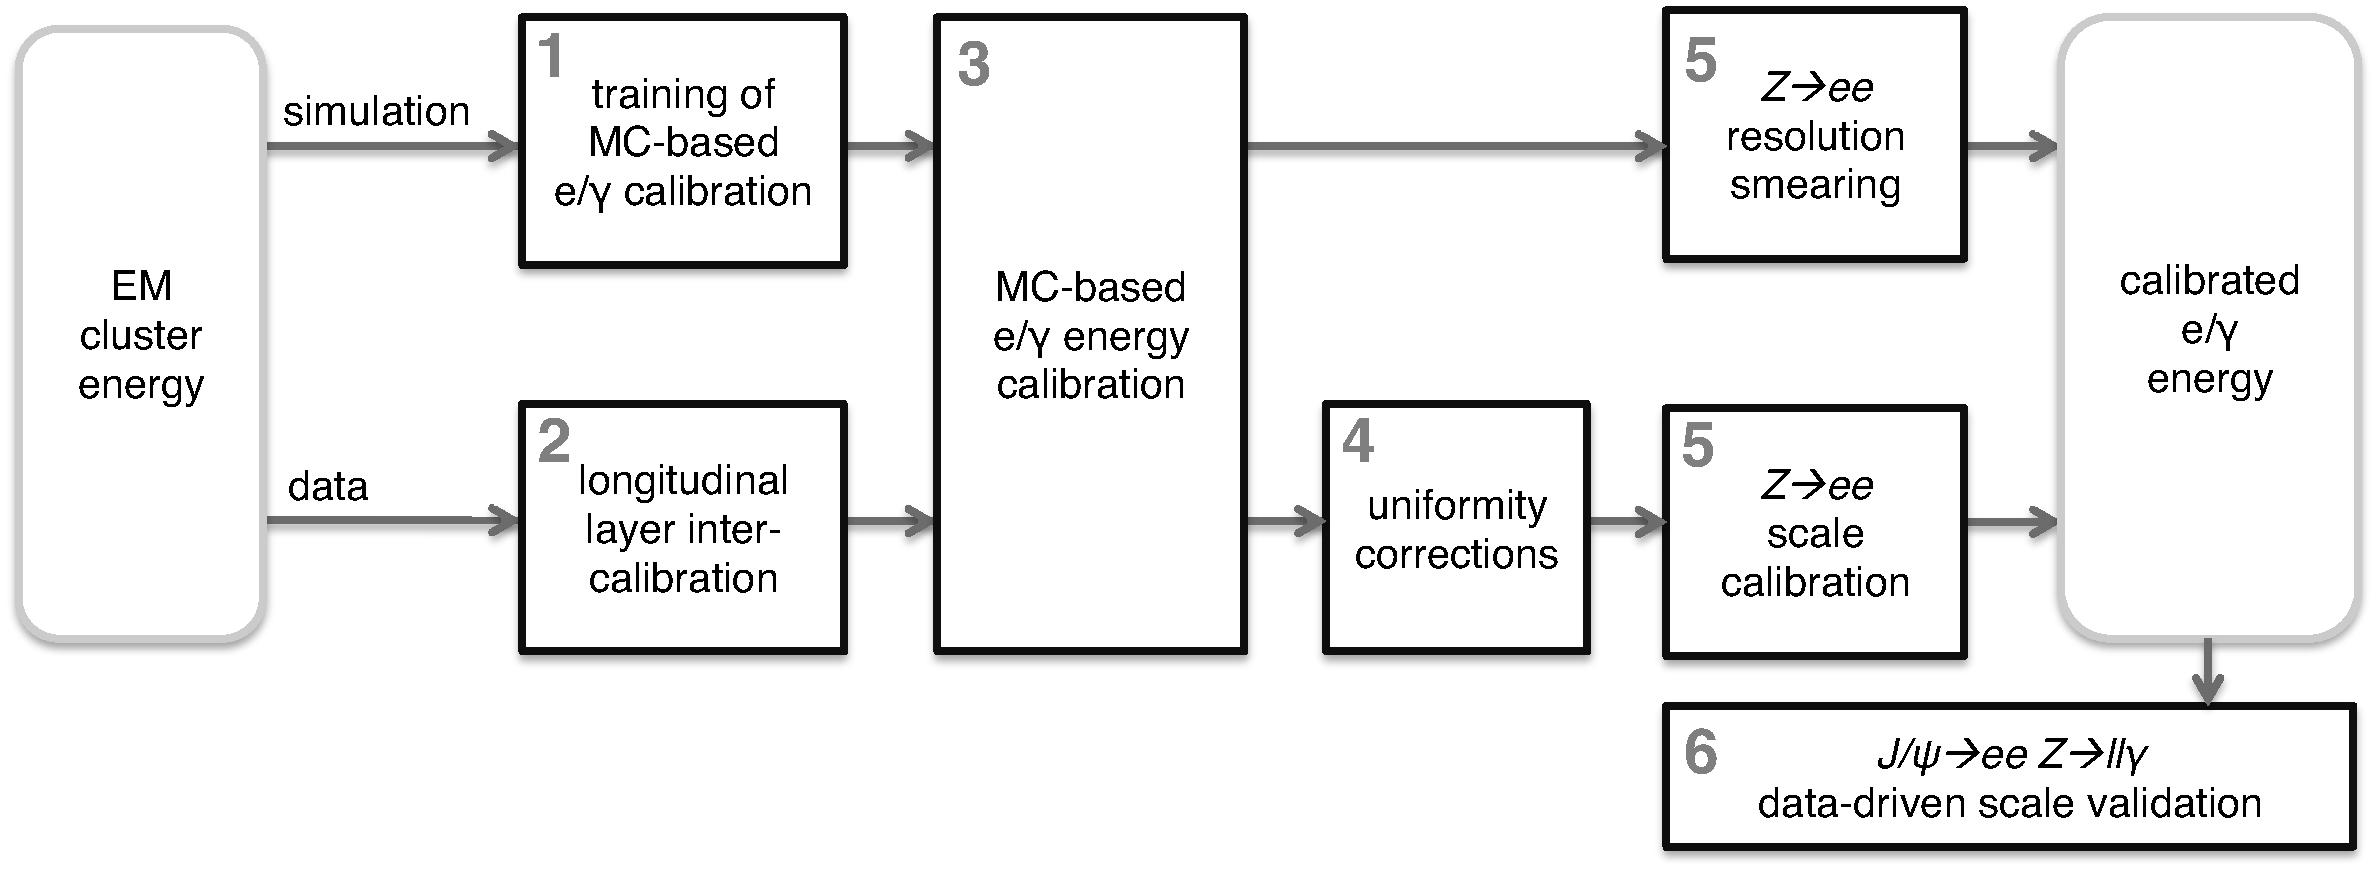
\includegraphics[width=0.8\columnwidth]{fig_01.png}
    	\caption{Schematic overview of energy response calibration procedure for electrons and photons.}
    	\label{fig:calibrationChain}
    \end{figure}
    In order to obtain the energy scale and resolution corrections the electrons from $Z\rightarrow ee$ process were used. The selection criteria were the same for data and MC simulation. For high-$\mu$ electron candidates must pass the triggers HLT\_2e12\_lhloose\_L12EM10VH (2015), HLT\_2e17\_lhvloose\_nod0 (2016), HLT\_2e24\_lhvloose\_nod0 (2017) and HLT\_2e24\_lhvloose\_nod0 (2018)~\cite{Aaboud:2018ugz}. In low pile-up case electron candidates must pass the triggers HLT\_e15\_lhloose\_nod0\_L1EM12. Both electrons are required to have $\pt > 27\,\GeV$ and |$\eta$| < 2.47, satisfying the medium LH ID criteria and loose isolation criteria as described in Ref.~\cite{PERF-2017-03}. 
    Energy scale correction follows the method described in detail in \cite{egamma_perf_2017} and schematically described in Fig. \ref{fig:calibrationChain}. The scale in both data and MC is calibrated using the MVA-based algorithm, then the data is corrected for pile-up and uniformity. The energy response in data is calibrated using the \Zee peak to match exactly the Z resonance in the simulation. Two correction factors are introduced: the energy scale factor $\alpha$ and the constant term $c'$. The correction factors are extracted using the template method described in Ref.~\cite{PERF-2013-05}:
    \begin{itemize}
    	\item The calorimeter is split into $i$ slices in $\eta$ and for each slice the energy response in data is corrected in the following way:
    	\begin{equation*}
    		E^{data,corr}=E^{MC}=E^{data,uncorr}/(1+\alpha_i),
    	\end{equation*}
    	where $E^{data,uncorr}$ and $E^{MC}$ are the energy response in data and MC respectively, $\alpha_i$ is the energy correction factor for the $i^{th}$ calorimeter slice in $\eta$.
    	\item The relative energy measurement resolution can be represented as a quadratic sum of three uncorrelated terms:
    	\begin{equation*}
    	\frac{\sigma(E)}{E}=\frac{a}{\sqrt{E}} \oplus \frac{b}{E} \oplus c,
    	\end{equation*}
    	where $b$ term stands for electromagnetic and pile-up noise term, $a$ is the stochastic term related to the development of the electromagnetic shower and $c$ is constant. In order to widen the MC mass peak and match it to the data in each rapidity bin an additional constant term $c'$ is added: 
    	\begin{equation*}
    	\left(\frac{\sigma(E)}{E}\right)^{data}_i= \left(\frac{\sigma(E)}{E}\right)^{MC}_i \oplus c_i'.
    	\end{equation*}
    \end{itemize}

Normally in the standard high-pileup data, the energy scale factors corrections are obtained in 68 $\eta$ bins.
For the low pile-up runs smaller bins were also considered due to smaller number of \Zee events. 
Figure~\ref{fig:alpha-lowmu-manybinnings} demonstrates the need for wider bins, as 68 bins result in high uncertainty, especially in the endcap.

Two binnings were considered:
\begin{itemize}
	\item 48 bins with smaller bins in the barrel and wider bins in the endcap
	\item 24 bins of equal size, as shown in Table~\ref{tab:lowmucalibbins}.
\end{itemize}
 As can be seen from Figure~\ref{fig:alpha-lowmu-manybinnings}, the
statistical instability for the endcap bins disappears if wider bins are used. 
Since the $\alpha$ factors are quite similar in 48 and 24 bin cases, the latter is chosen as the baseline.

\begin{table}
		\resizebox{\linewidth}{!}{%
		\begin{tabular}{c}
			\toprule
			-2.47 -2.4 -2.1 -1.8 -1.55 -1.37 -1.2 -1 -0.8 -0.6 -0.4 -0.2 0 0.2 0.4 0.6 0.8 1 1.2 1.37 1.55 1.8 2.1 2.4 2.47\\
			\bottomrule
		\end{tabular}%
	}
	\caption{Values of $\eta_{\text{calo}}$ bin frontiers for energy scale factors for low pile-up runs.}\label{tab:lowmucalibbins}
	\label{tab:CS_BinFrontier}
\end{table}

\begin{figure}[htp]
	\begin{center}
		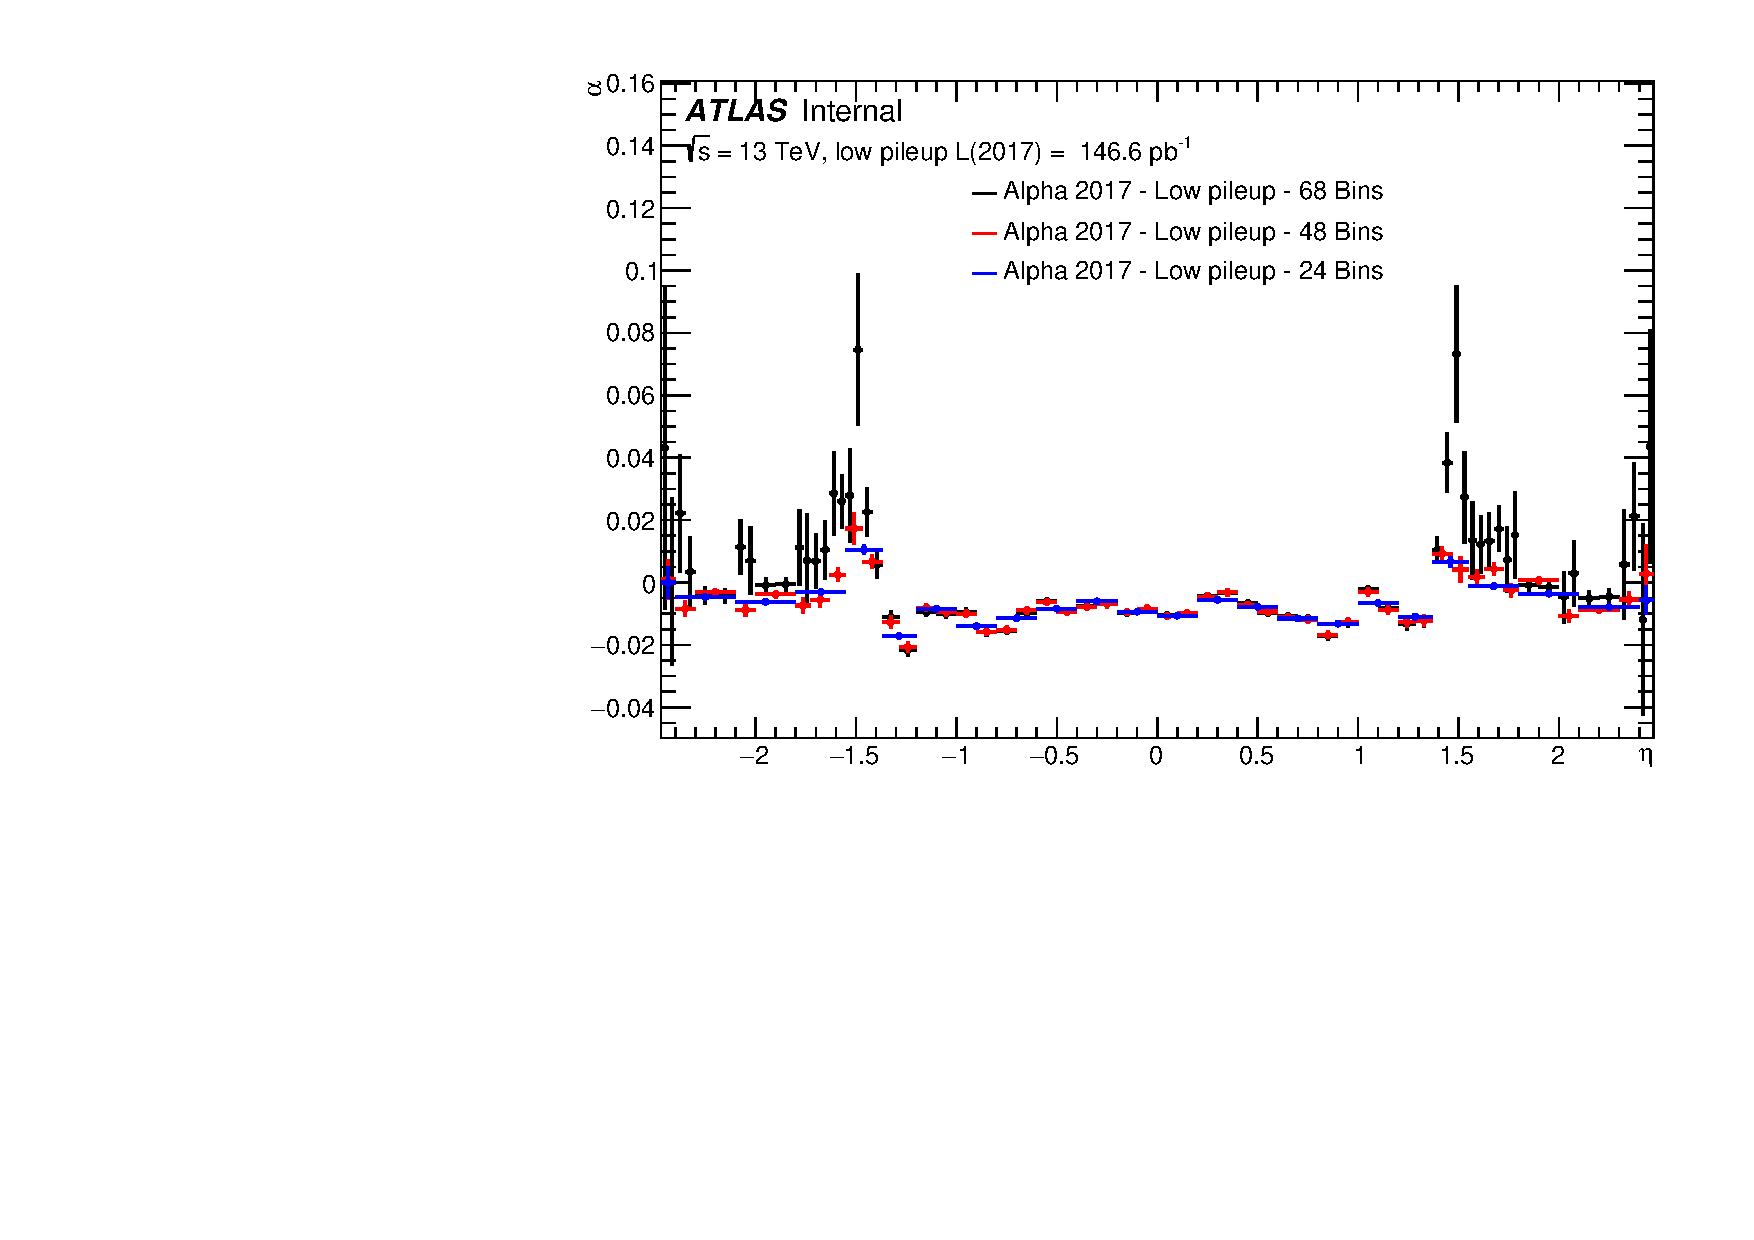
\includegraphics[width=0.5\linewidth]{Plot/low2017Bins.pdf}%
		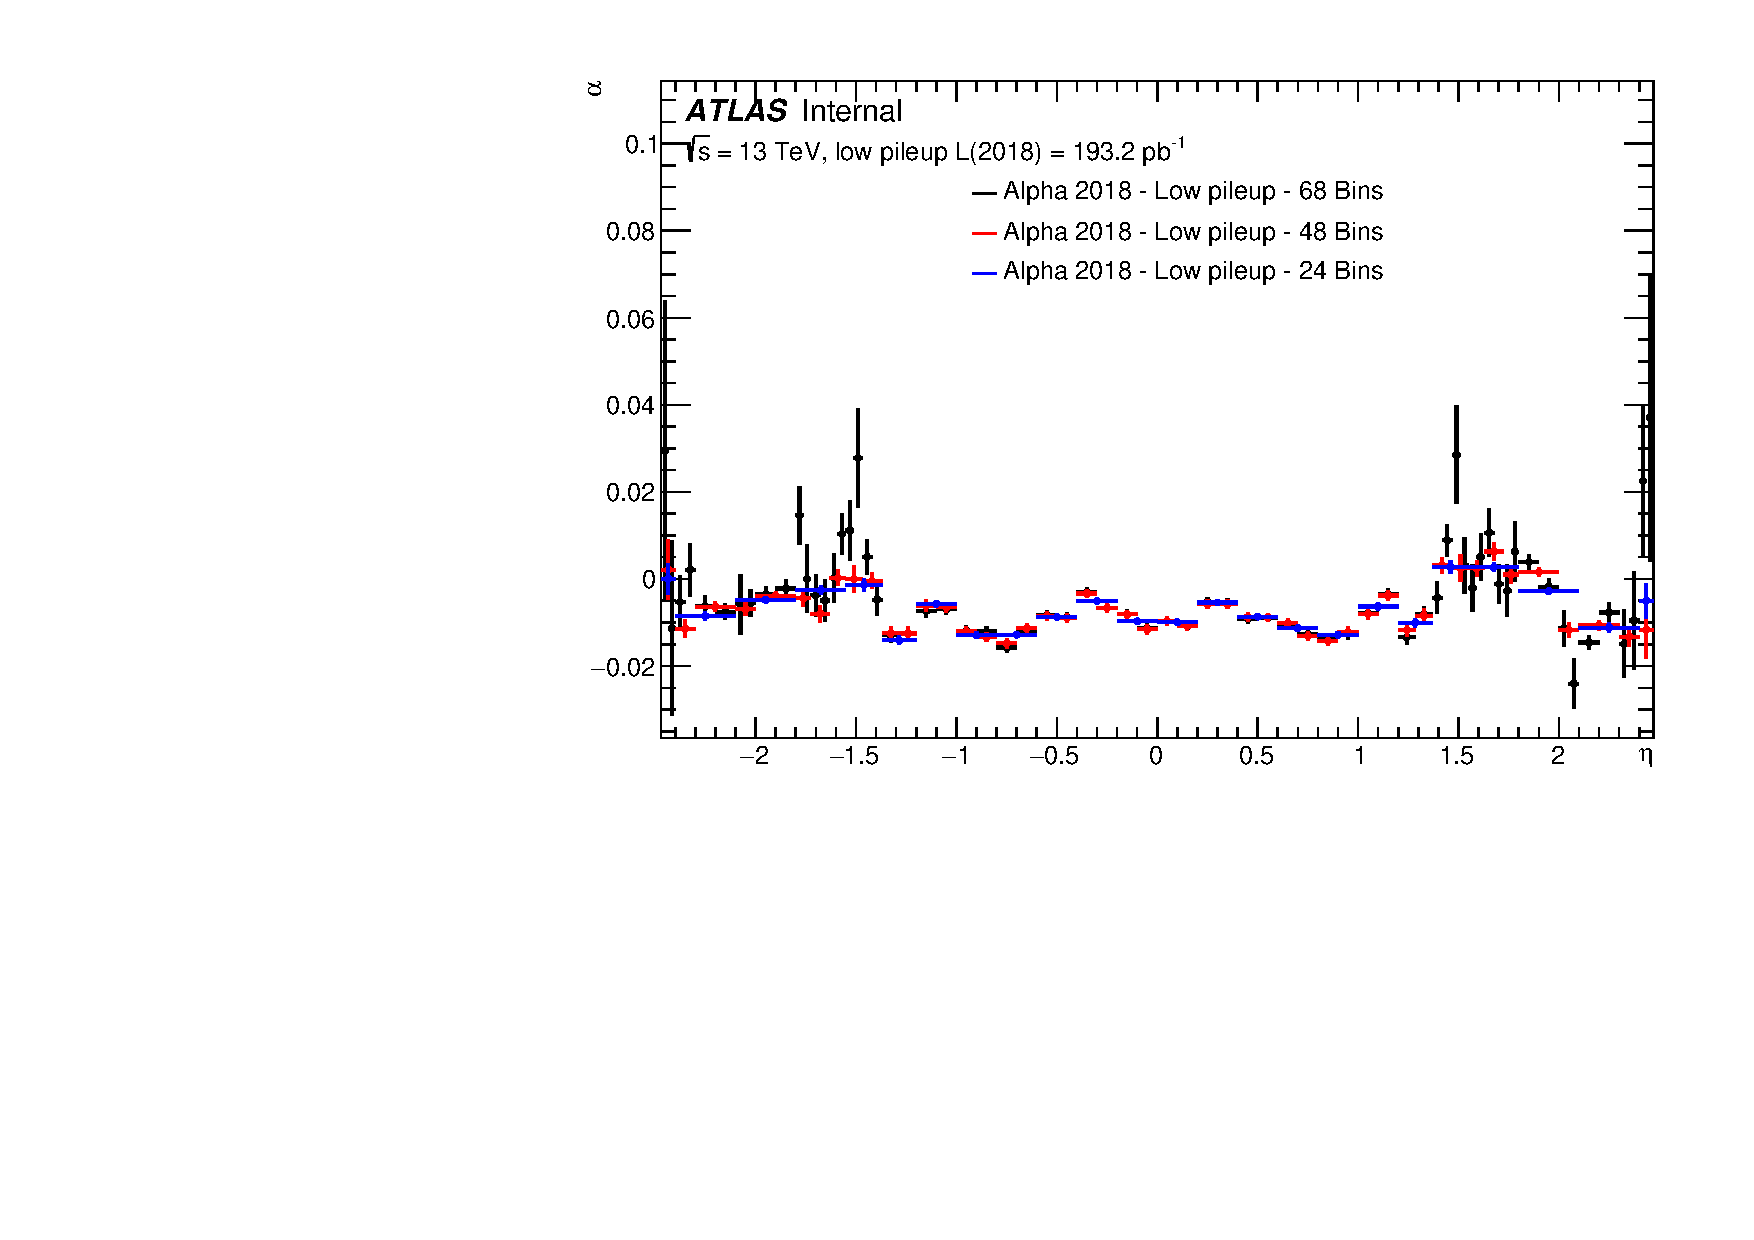
\includegraphics[width=0.5\linewidth]{Plot/low2018Bins.pdf}
		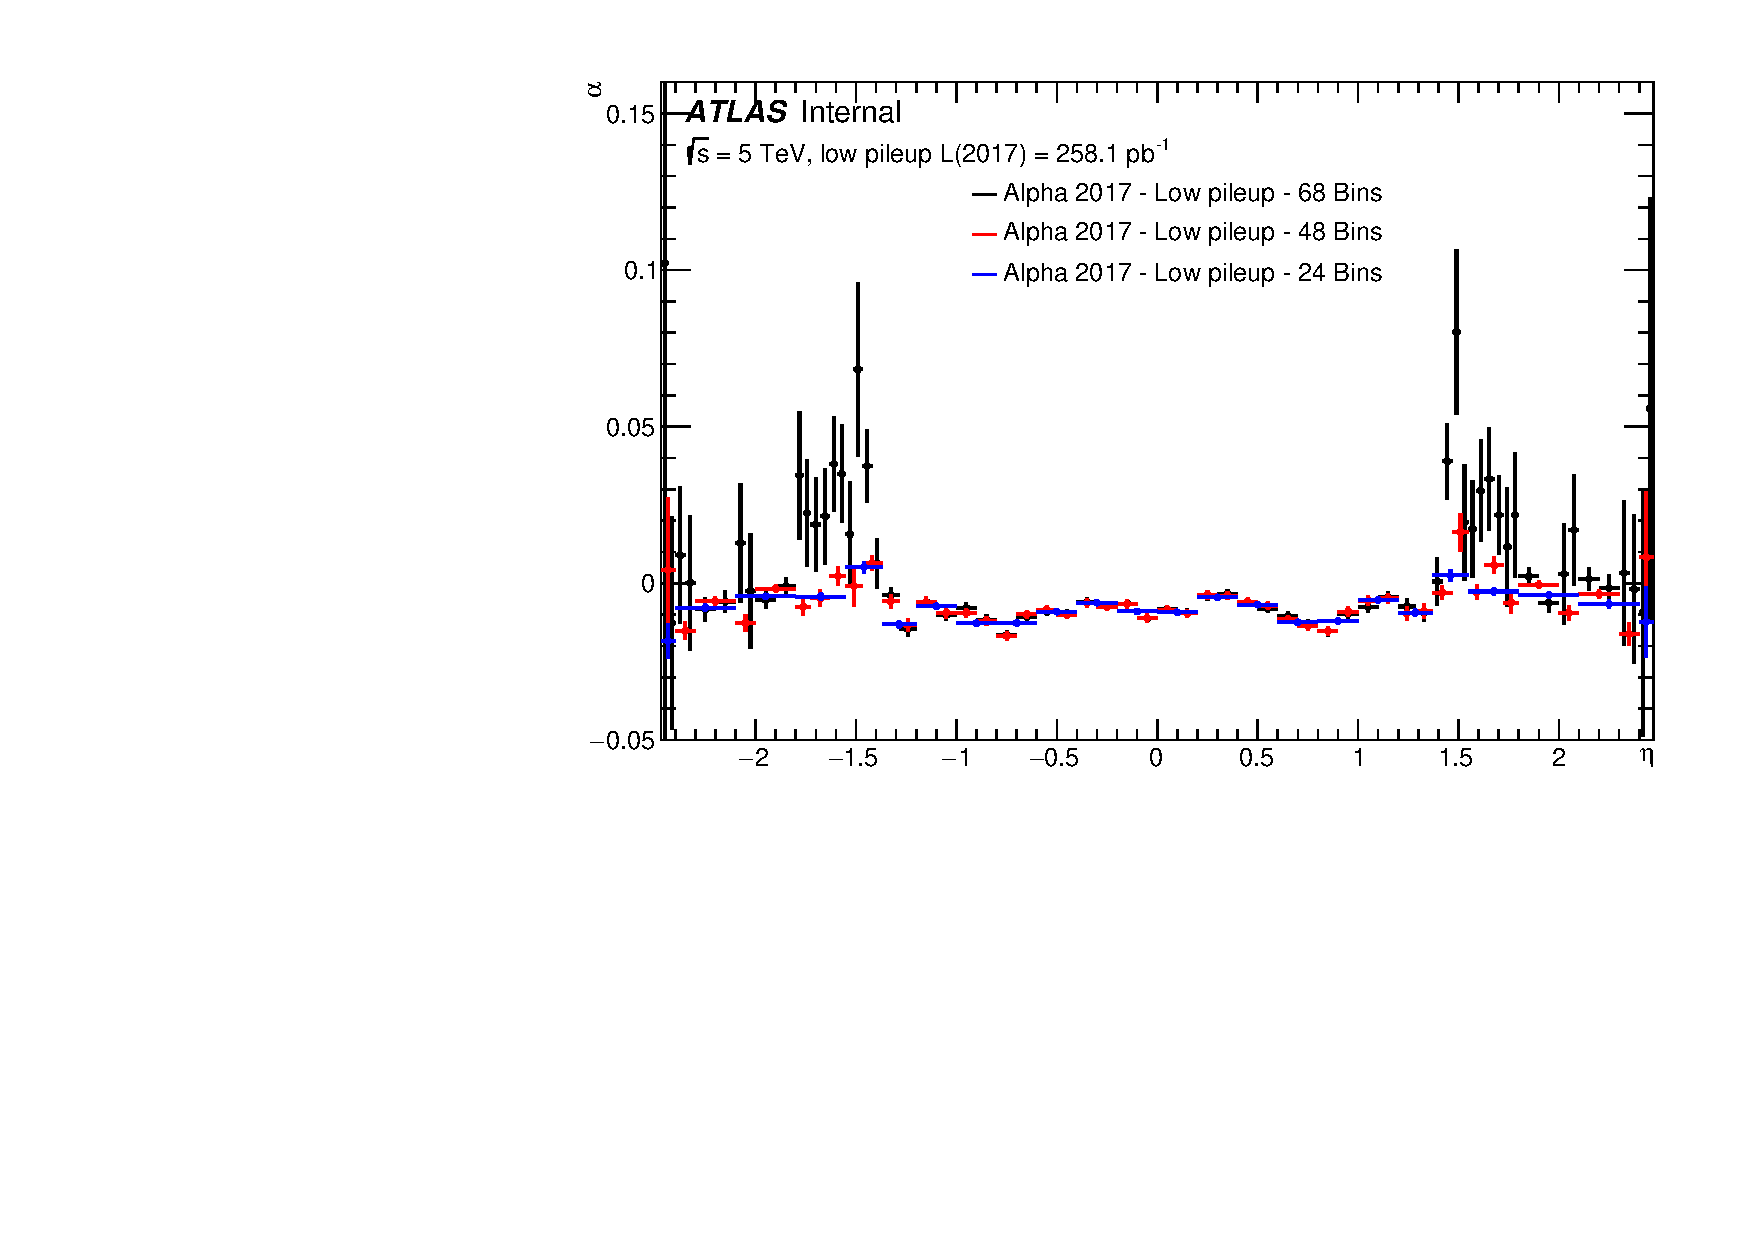
\includegraphics[width=0.5\linewidth]{Plot/low2017Bins_5TeV.pdf}
		\caption{ Energy scale factors $\alpha$ for low pile-up runs of
			2017 (left), 2018 (right) and 2017 at 5TeV (bottom) using 68, 48 and 24 $\eta$ 
			bins. It can be seen, that the extraction is unstable in case of 68 bins,
			resulting in $\alpha$ factors with very large uncertainties.}
		\label{fig:alpha-lowmu-manybinnings}
	\end{center}
\end{figure}

The extracted constant $c_i'$ correction term is presented in
Figure~\ref{fig:C_lowmu}. The constant term $c'$ depends on the data taking conditions and pile-up, so its extrapolation from a dataset obtained under different conditions appears problematic. This issue is discussed in Ref.~\cite{Andari:2651890}.

\begin{figure}[htp]
	\begin{center}
		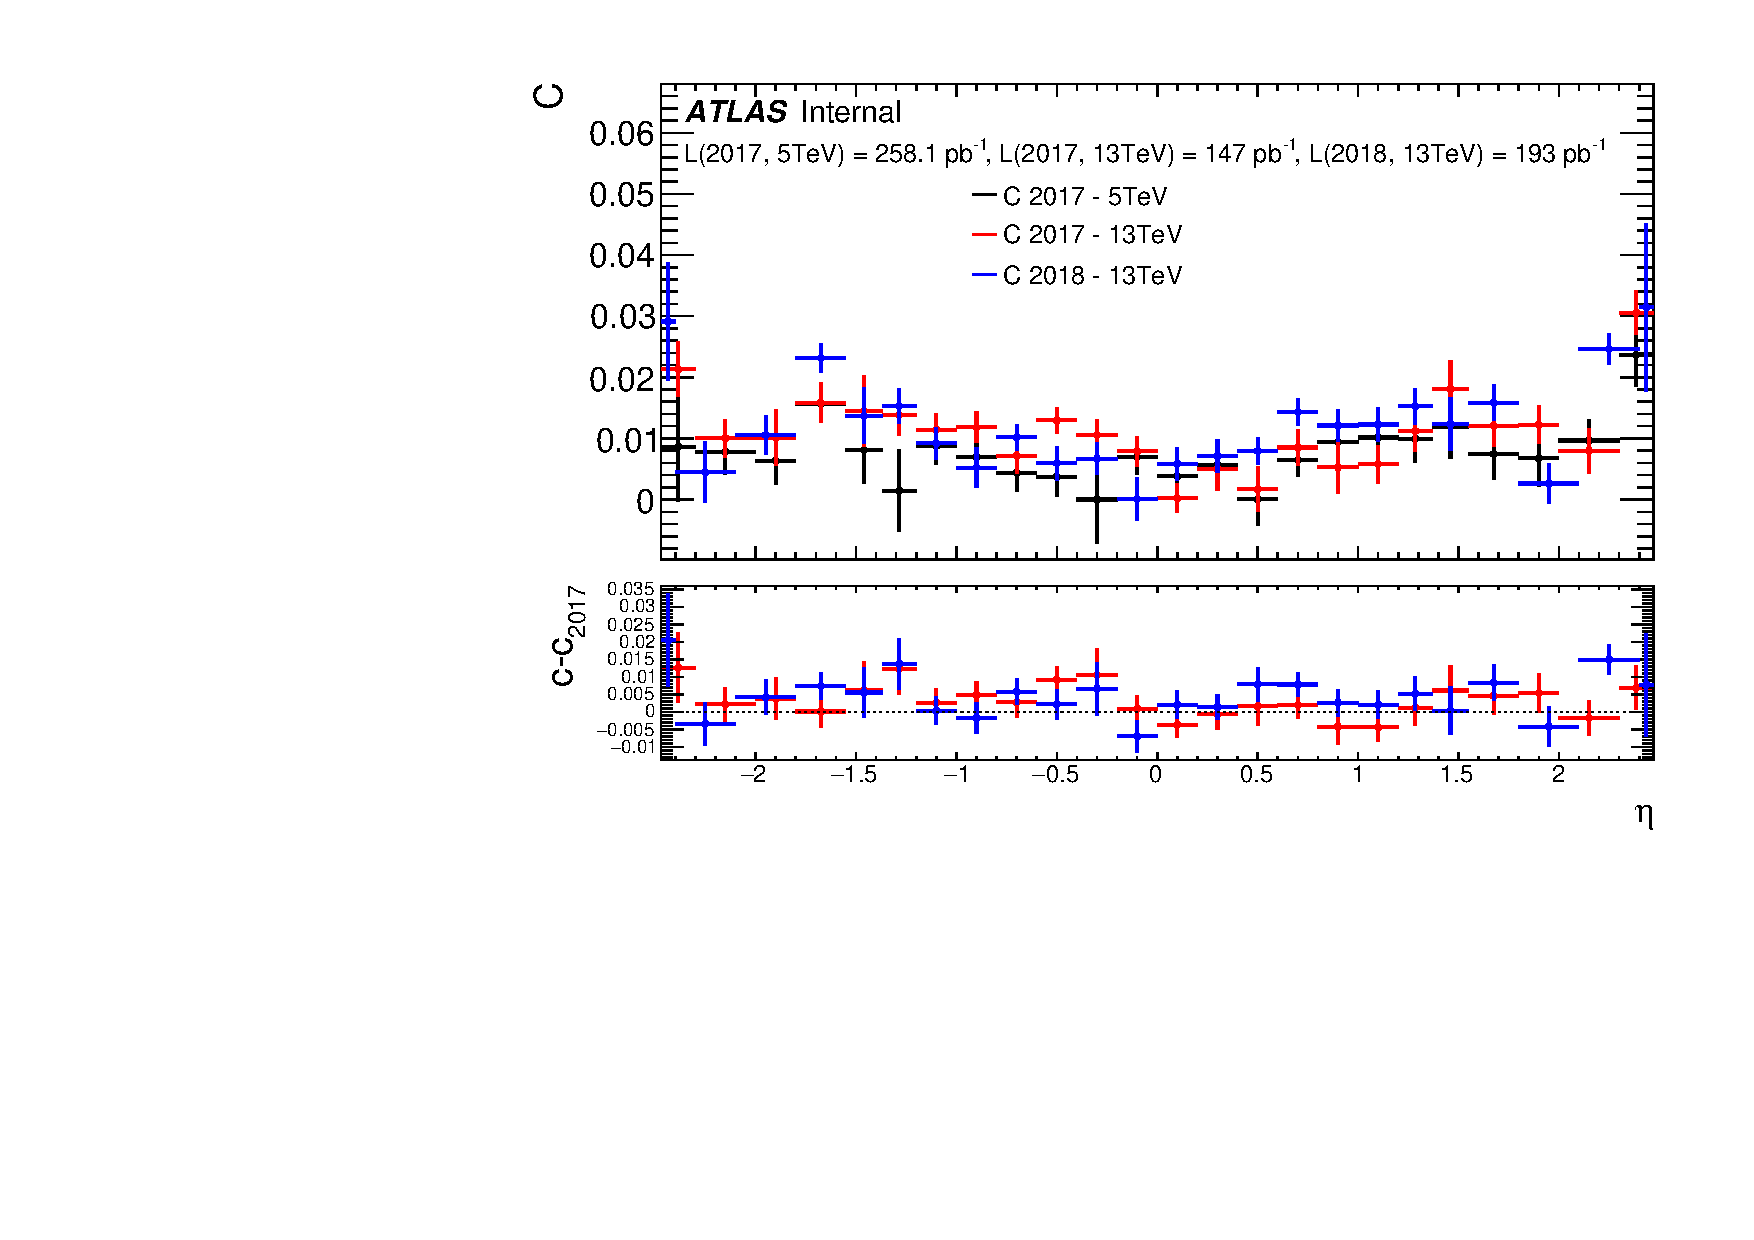
\includegraphics[width=0.5\linewidth]{Plot_C.pdf}%
		\caption{ Additional constant term $c_i'$ for low pile-up runs of 
			2017 (13 \TeV), 2018 (13 \TeV) and 2017 at 5 \TeV{} using 24 bins.
			The lower panel shows the difference of $c_i'$ to the 2017 5 TeV run.}
		\label{fig:C_lowmu}
	\end{center}
\end{figure}

This correction entails experimental uncertainty, caused primarily by the statistical uncertainty of $\alpha_i$ and $c_i'$ factors measurement, other uncertainties are significantly smaller and therefore neglected.\\
The comparison between data and MC invariant mass distributions around the \Zee peak are presented in Figure~\ref{fig:mee-lowmu-data-vs-MC} and Figure~\ref{fig:alpha-highmu-lowmu-thresh-corr}. The agreement is good around the \Zee resonance and stays within the uncertainty in other regions.

\begin{figure}[H]
	\center
	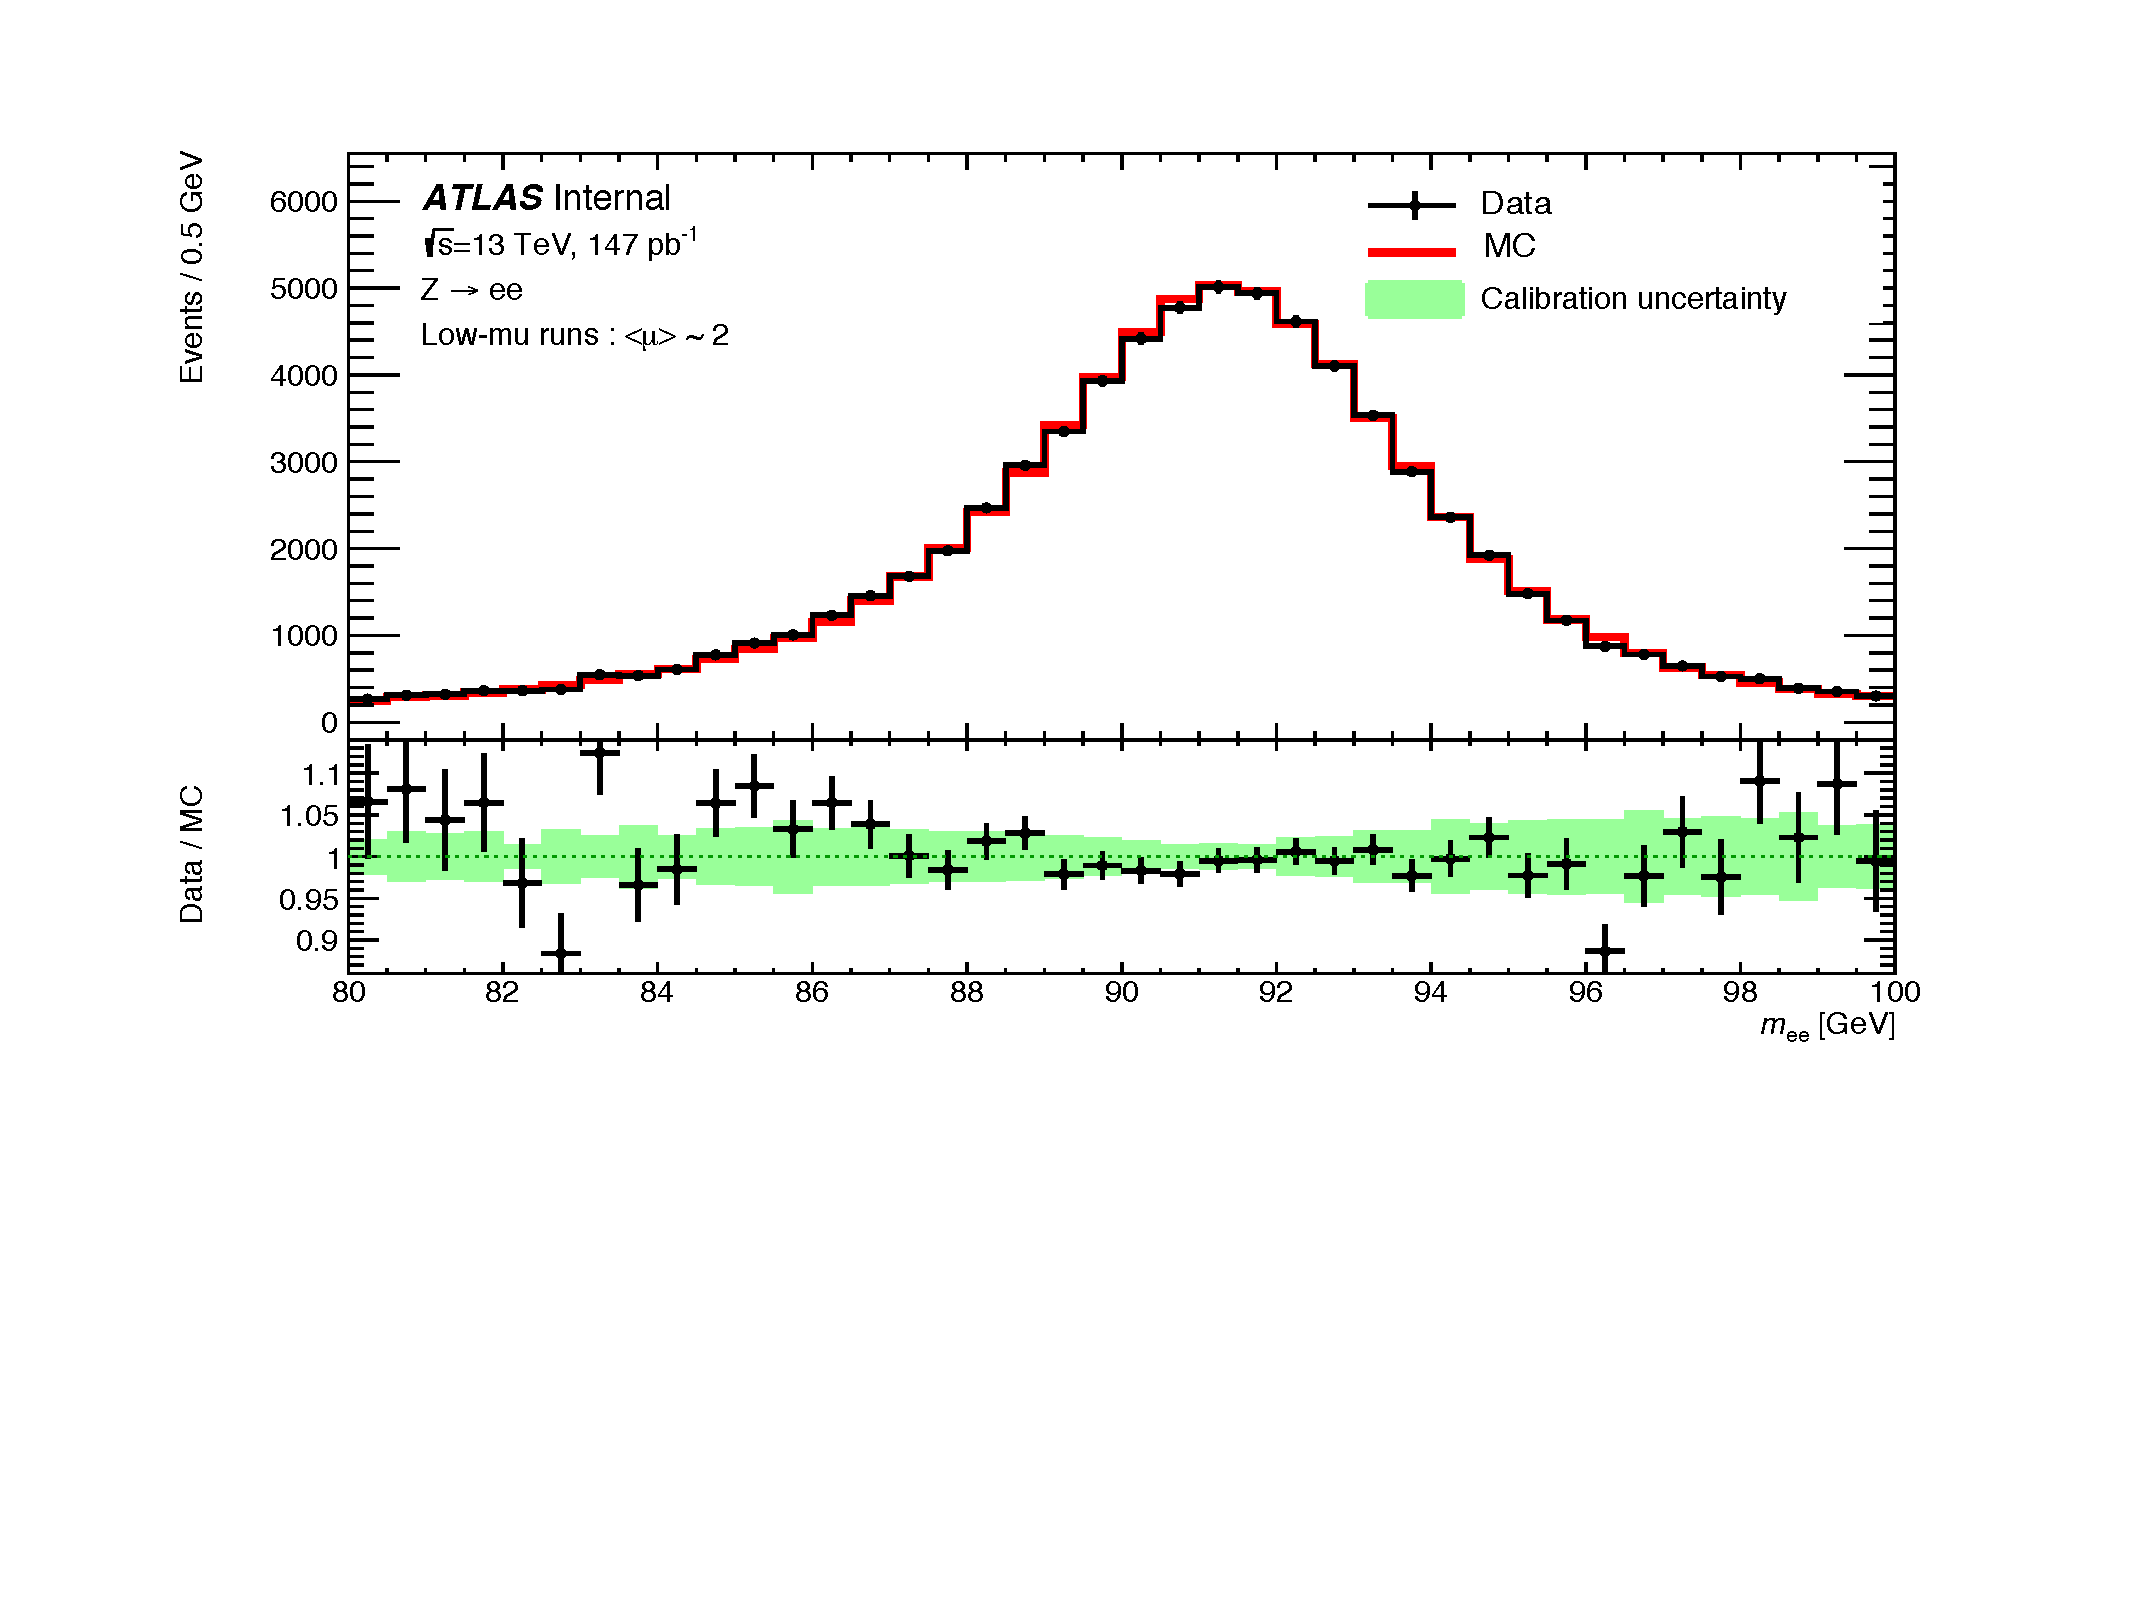
\includegraphics[width=14cm]{Plot/lowmuMee.pdf}
	\caption{The invariant mass distribution around the Z-mass for low pile-up Data for 2017 (13 TeV)}
	\label{fig:mee-lowmu-data-vs-MC}
\end{figure}
\begin{figure}[H]
\begin{center}
    {{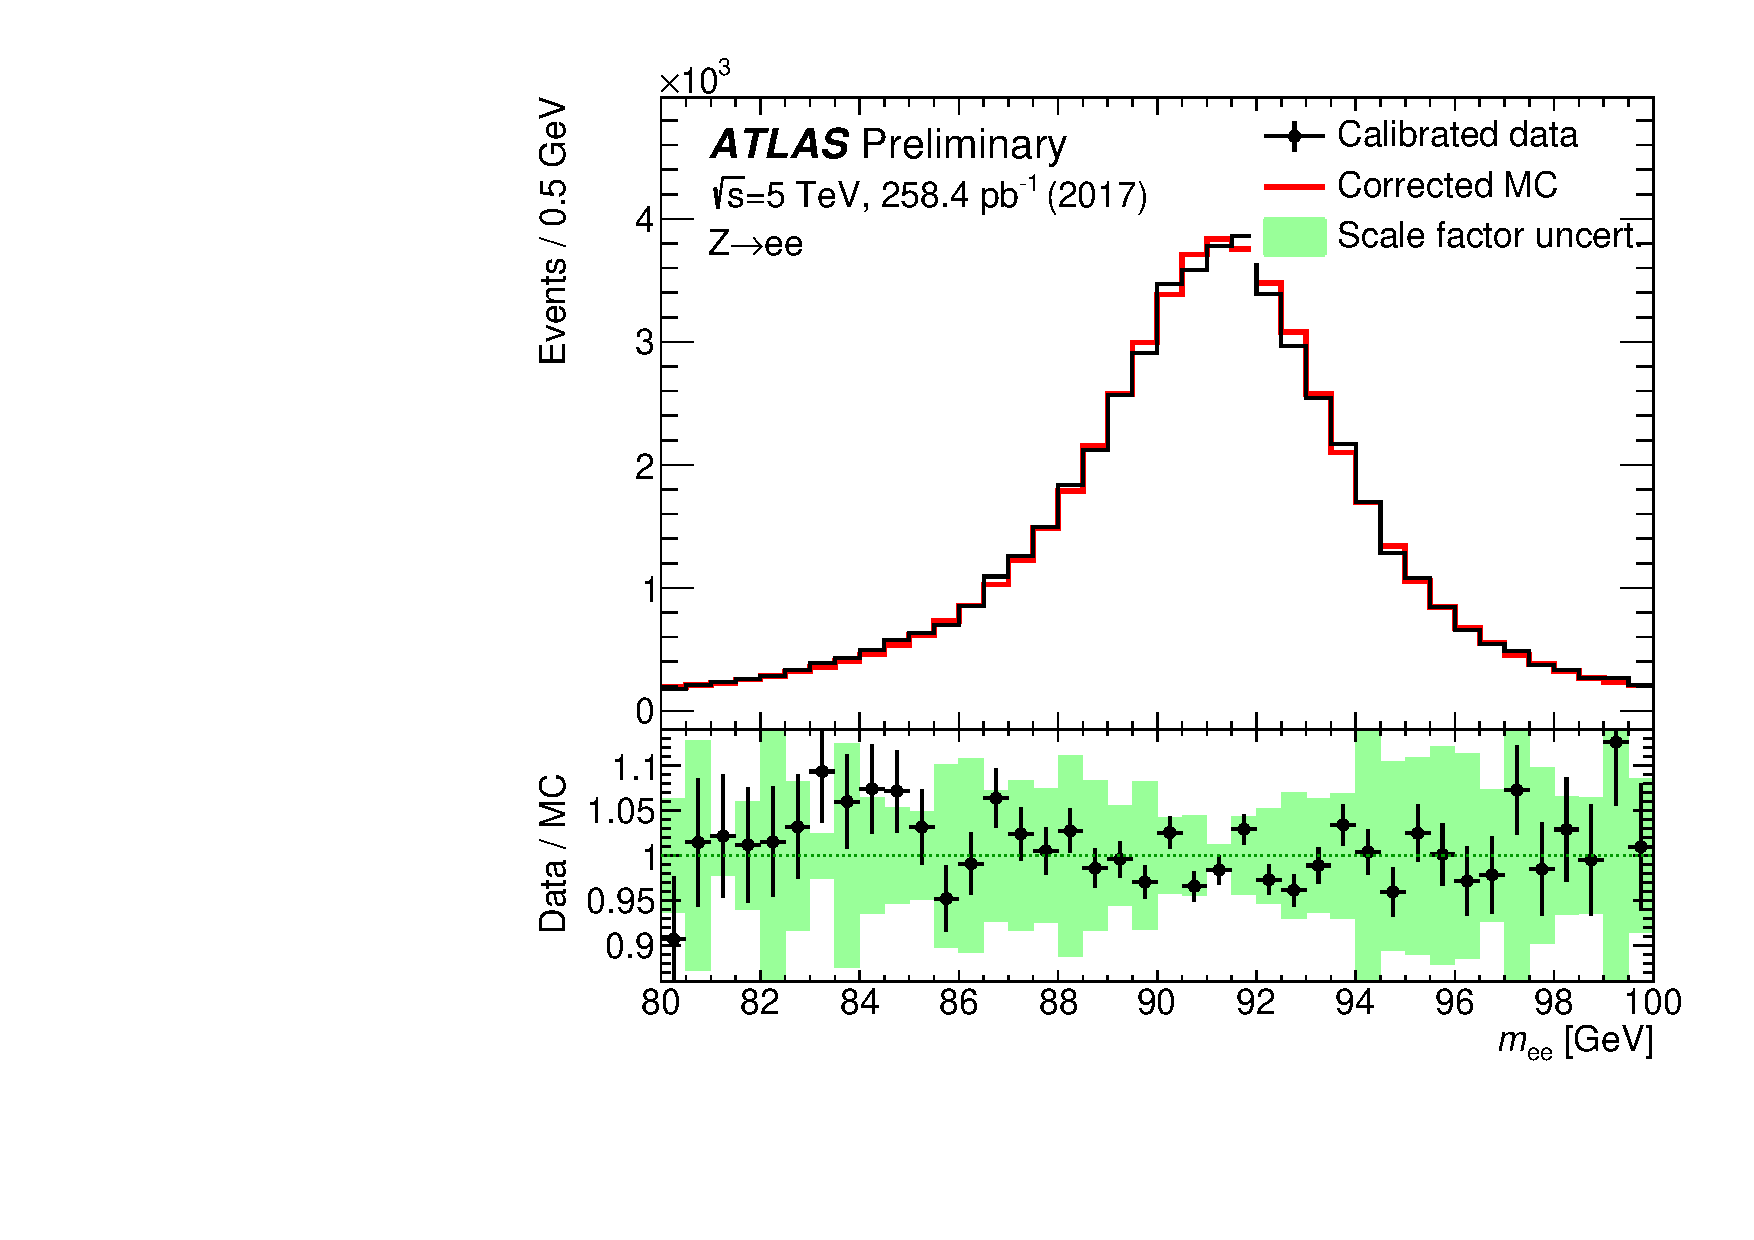
\includegraphics[width=0.48\linewidth]{ZeeMass_corrected_2017_5TeV.pdf}
    }}
    {{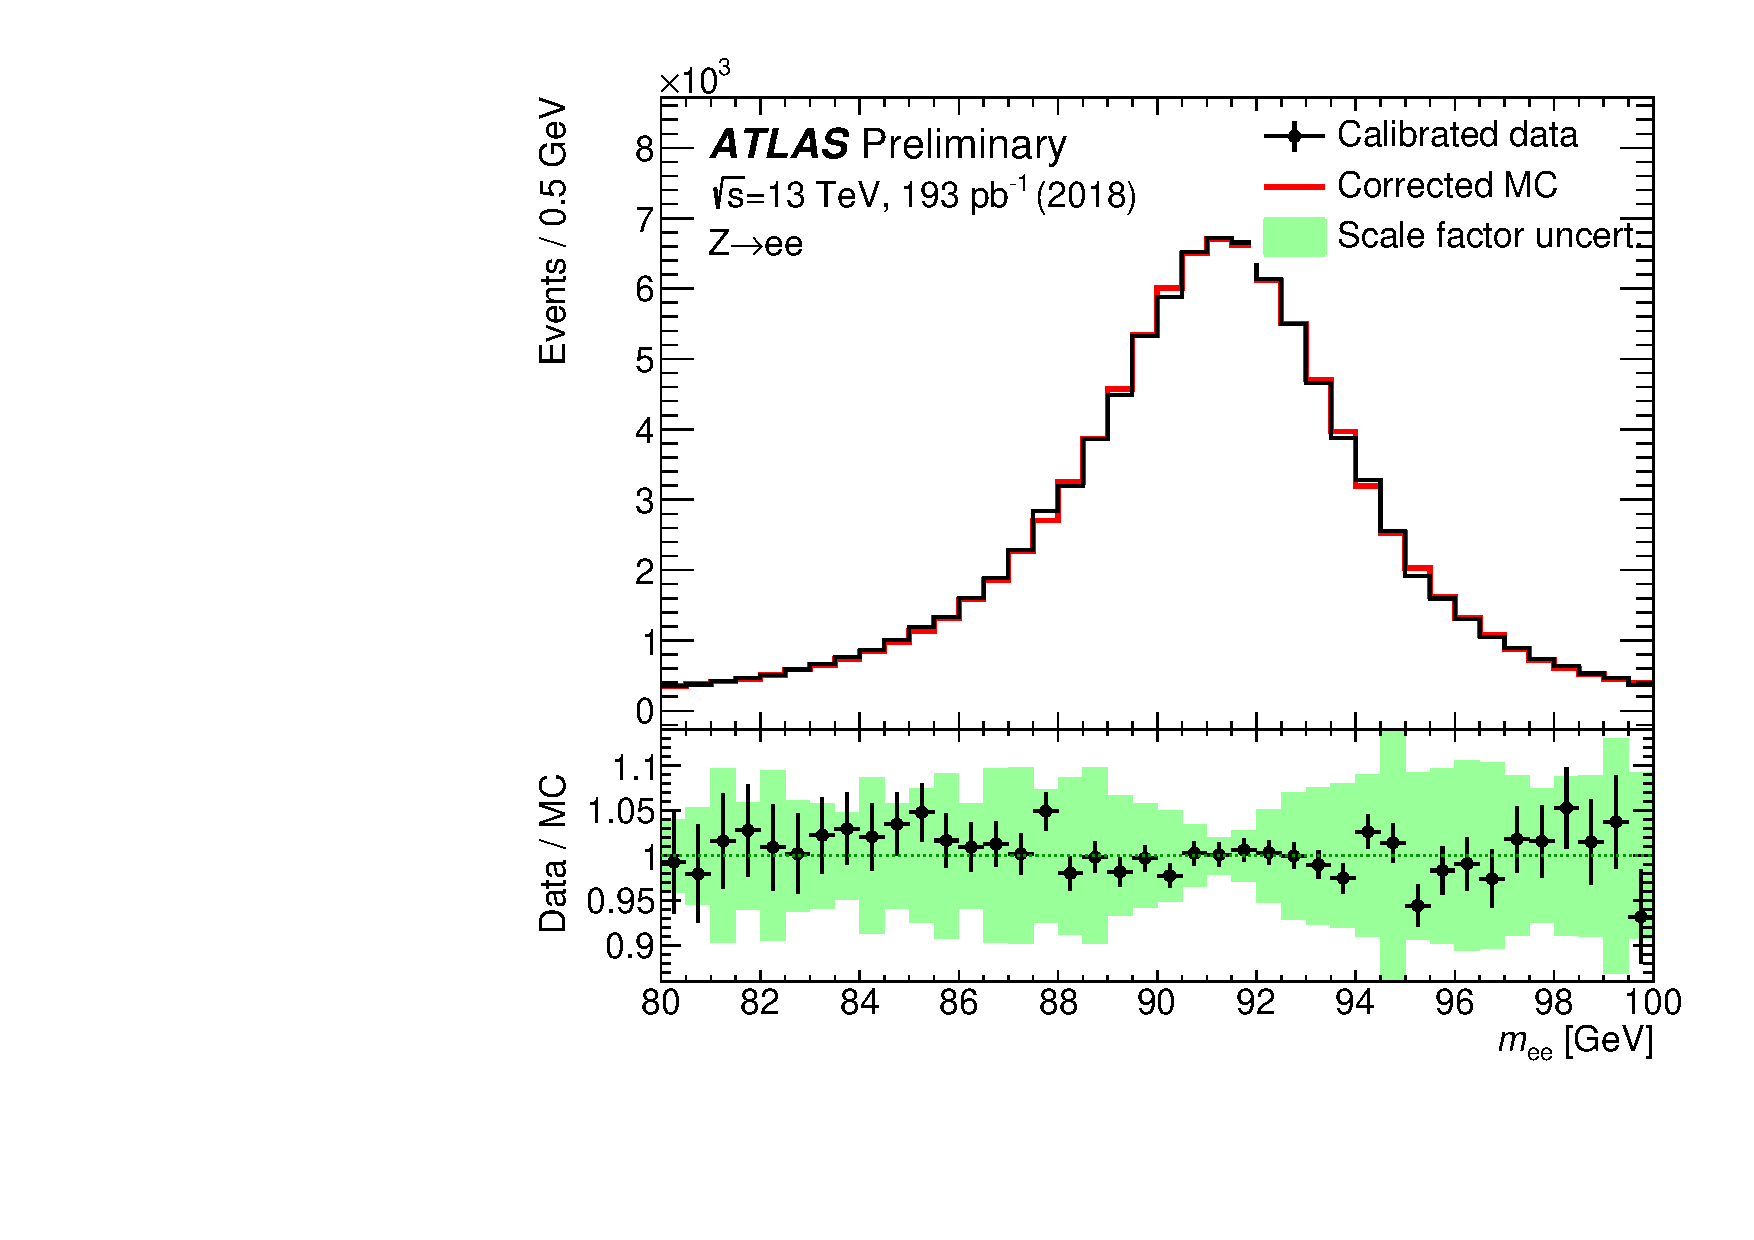
\includegraphics[width=0.48\linewidth]{ZeeMass_corrected_2018.pdf}
    }}
    \caption{ The invariant mass distribution around the Z-mass for low-pileup data for the $\sqrt{s}=5\,\TeV$ data taken in 2017 (a) and the $\sqrt{s}=13\,\TeV$ 2018 data (b).}
    \label{fig:alpha-highmu-lowmu-thresh-corr}
\end{center}
\end{figure}

\clearpage
	
    \subsection{Electron selection efficiency}
    The electrons used in the analysis are selected based on certain requirements to the quality of their reconstruction, kinematic characteristics, passing certain identification, isolation and trigger matching criteria. A tag-and-probe method is used to measure these efficiencies in data and MC simulation, which may be different due to various aspects of physics and detector modelling. In order to match the MC simulation and the data in each of the aforementioned aspects the corresponding \gls{sf}s are introduced. The SF is defined as the ratio of the data efficiency to MC efficiency:
     \begin{equation*}
     SF_{(a)}=\frac{\epsilon^{data}_{(a)}}{\epsilon^{MC}_{(a)}},
     \end{equation*}
     where $\epsilon$ stand for efficiency and index $a$ stands for reconstruction, ID, isolation or trigger. The \gls{sf} extraction allows for better comparison between data and simulation, but also brings uncertainties. The total efficiency correction is used as an event weight during the analysis:
     \begin{equation*}
     W_{event}^{W\rightarrow e\nu}=SF_{reco} \dot SF_{trig} \dot SF_{ID} \dot SF_{iso}.
     \end{equation*}
     The tag-and-probe method used for the measurement of electron efficiencies includes the following steps:
     \begin{itemize}
     	\item A kinematic selection is applied to \Zee events (Cut1).
     	\item A tight selection (Cut2) is applied to one of the two electrons along with matching it to the single-electron trigger. From now on this electron is called the \textit{tag}.
     	\item The other electron is called the \textit{probe} and is used to probe the picked efficiency.
     	\item Selections Cut1 and Cut2 are varied in order to evaluate the uncertainties. 
     \end{itemize}
 	The details are presented in Refs. \cite{Aaboud:2018ugz, electrons_reco1, topoclust_2019}.
    \subsubsection{Reconstruction efficiency}
    The reconstruction efficiency is defined as a fraction of all electromagnetic clusters that are matched with the charged particle track from the \gls{id} that matches the designated quality criteria. An additional "PassTrackQuality" requirement of having at least 1 hit in the pixel detector and and least 7 hits in the silicon detectors is imposed on the track of successfully reconstructed electrons. \\
    So the electron reconstruction efficiency is calculated as:
    \begin{equation}
    \label{eq:eff_reco}
    \epsilon^{reco}(p_T,\eta)=\frac{N_{pass}-N_{pass}^{bkg}}{N_{pass}-N_{pass}^{bkg}+N_{fail}-N_{fail}^{bkg}+N_{photon}-N_{fit}}.
    \end{equation}
    $N_{pass(fail)}$ stands for the number of electrons passing (failing) the "PassTrackQuality" criterion. The background electron candidates $N^{bkg}_{pass(fail)}$ are obtained from the template fits of the background on subsets that pass (fail) the "PassTrackQuality" criterion. The number of electrons that are reconstructed as photons is denoted by $N_{photon}$. The non-electron background that is reconstructed as photons is estimated from analytical fit in the control region away from the \Zee resonance and is called $N_{fit}$.\\
    An extrapolation of $SF_{reco}$ from the high-$\mu$ data is used as a baseline for the reconstruction scale factors measurement. The benefits of higher statistics available in high-$\mu$ dataset outweigh the losses imposed by the extrapolation and provide lower uncertainty comparing to the SFs measured with low pileup dataset (see Fig. \ref{fig:extra_sys_13_medium}).
    \begin{figure}[htbp]
    	\begin{center}
    		\includegraphics[width=0.48\textwidth]{Efficiencies/Reco/extra/Uncer/13TeV/syspt}
    		\includegraphics[width=0.48\textwidth]{Efficiencies/Reco/extra/Uncer/13TeV/syseta}
    		\includegraphics[width=0.48\textwidth]{Efficiencies/Reco/extra/Uncer/13TeV/sys_met}
    		\includegraphics[width=0.48\textwidth]{Efficiencies/Reco/extra/Uncer/13TeV/sys_mT}
    	     \includegraphics[width=0.48\textwidth]{Efficiencies/Reco/extra/Uncer/13TeV/boson_pT}
    		\caption{Comparison of the uncertainties due to electron
    			reconstruction, contrasting the high-$\mu$-extrapolated and
    			in-situ-measured SF uncertainties in a $W^{+}\rightarrow
    			e^{+}\nu$ selection at 13 TeV as function of typical kinematic variables.}
    		\label{fig:extra_sys_13_medium}
    	\end{center}
    \end{figure}
    \clearpage
    \subsubsection{Identification efficiency}
    The fraction of reconstructed electrons that pass a given working point define the electron identification efficiency. The low pile-up \Wen measurement uses "Medium LH" working point. The methodology is described in Ref. \cite{electrons_reco1} and includes the combination of two background subtraction methods: \textit{Zmass} and \textit{Ziso}. \\
    In the Zmass method the background is estimated using a template method normalized in $m_{ee}$ side bands. The tag is required to be trigger-matched, pass ID and isolation cuts and have $p_T>20$ GeV. The probe has to pass the "PassTrackQuality" and the electron/photon ambiguity resolver, have $p_T>15$ GeV and be separated from jets with $p_T^{jet}>20$ GeV by $\Delta R>0.4$.\\
    An alternative $Ziso$ method uses the calorimeter energy isolation $E_T^{cone}$ of the probe electron to discriminate between background and signal. Signal electrons are expected to have better isolation than the background. On top of the requirements used for the Zmass method the tag and probe pair is required to have opposite sign and to fit into mass window of 15 GeV around the Z boson mass. Background template shape is constructed from the probe electrons that have the same charge as the tag, pass the track quality criteria but fail the shower shape cuts or fail the cut-based loose identification. The fraction of real electrons that pass the described selection is modelled with MC and subtracted from the template. The background template uses the tail region of probe isolation distribution $E_T^{cone0.3}/25\gev > 0.5$ is scaled to data events. An example of the probe isolation estimate for the enumerator and denominator in eq. \ref{eq:eff_reco} in the region $25<E_T<30$ and $0.8<\eta<1.15$ is presented in Fig. \ref{fig:bkgfit_ziso}.
    
    \begin{figure}[htbp]
    \centering
    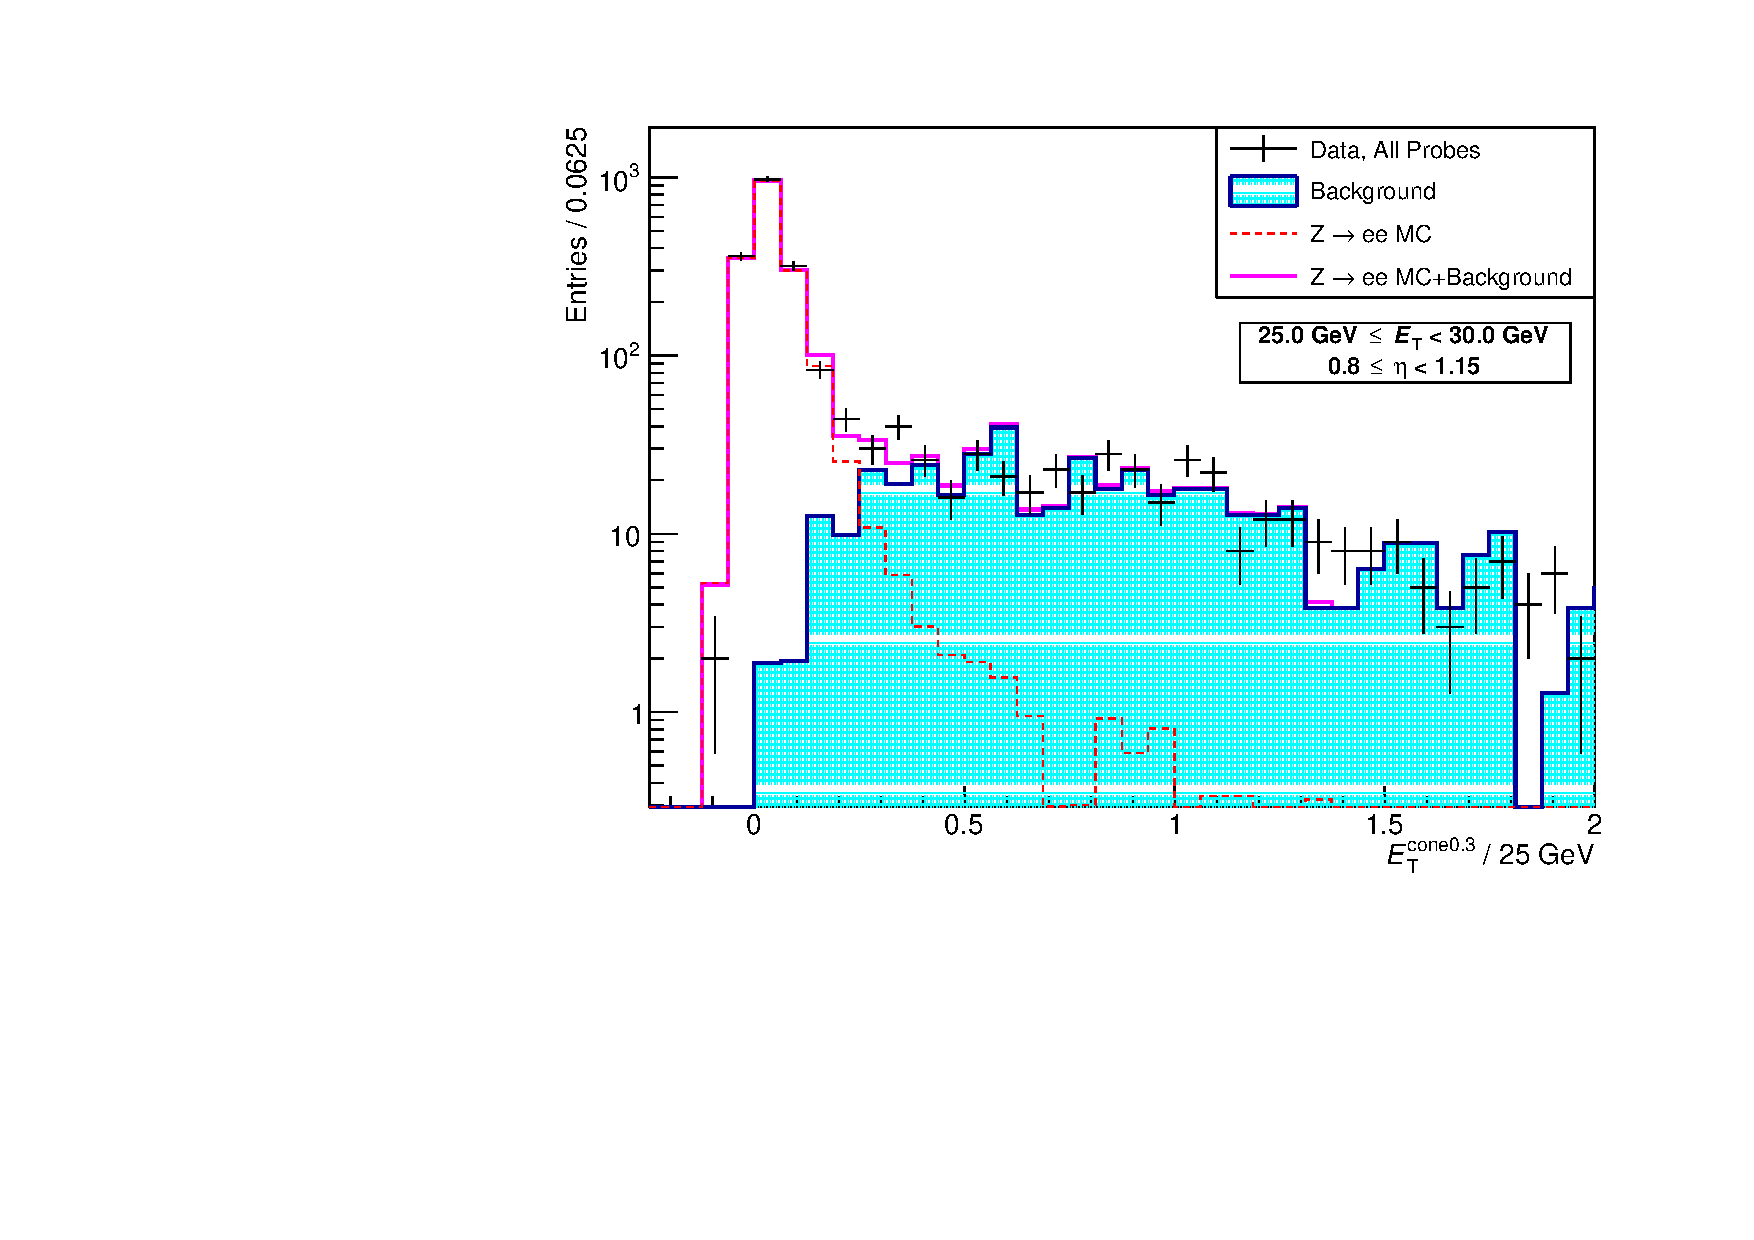
\includegraphics[width=0.48\textwidth]{Efficiencies/ID/Bkg_Den_13TeV_ZIso}
    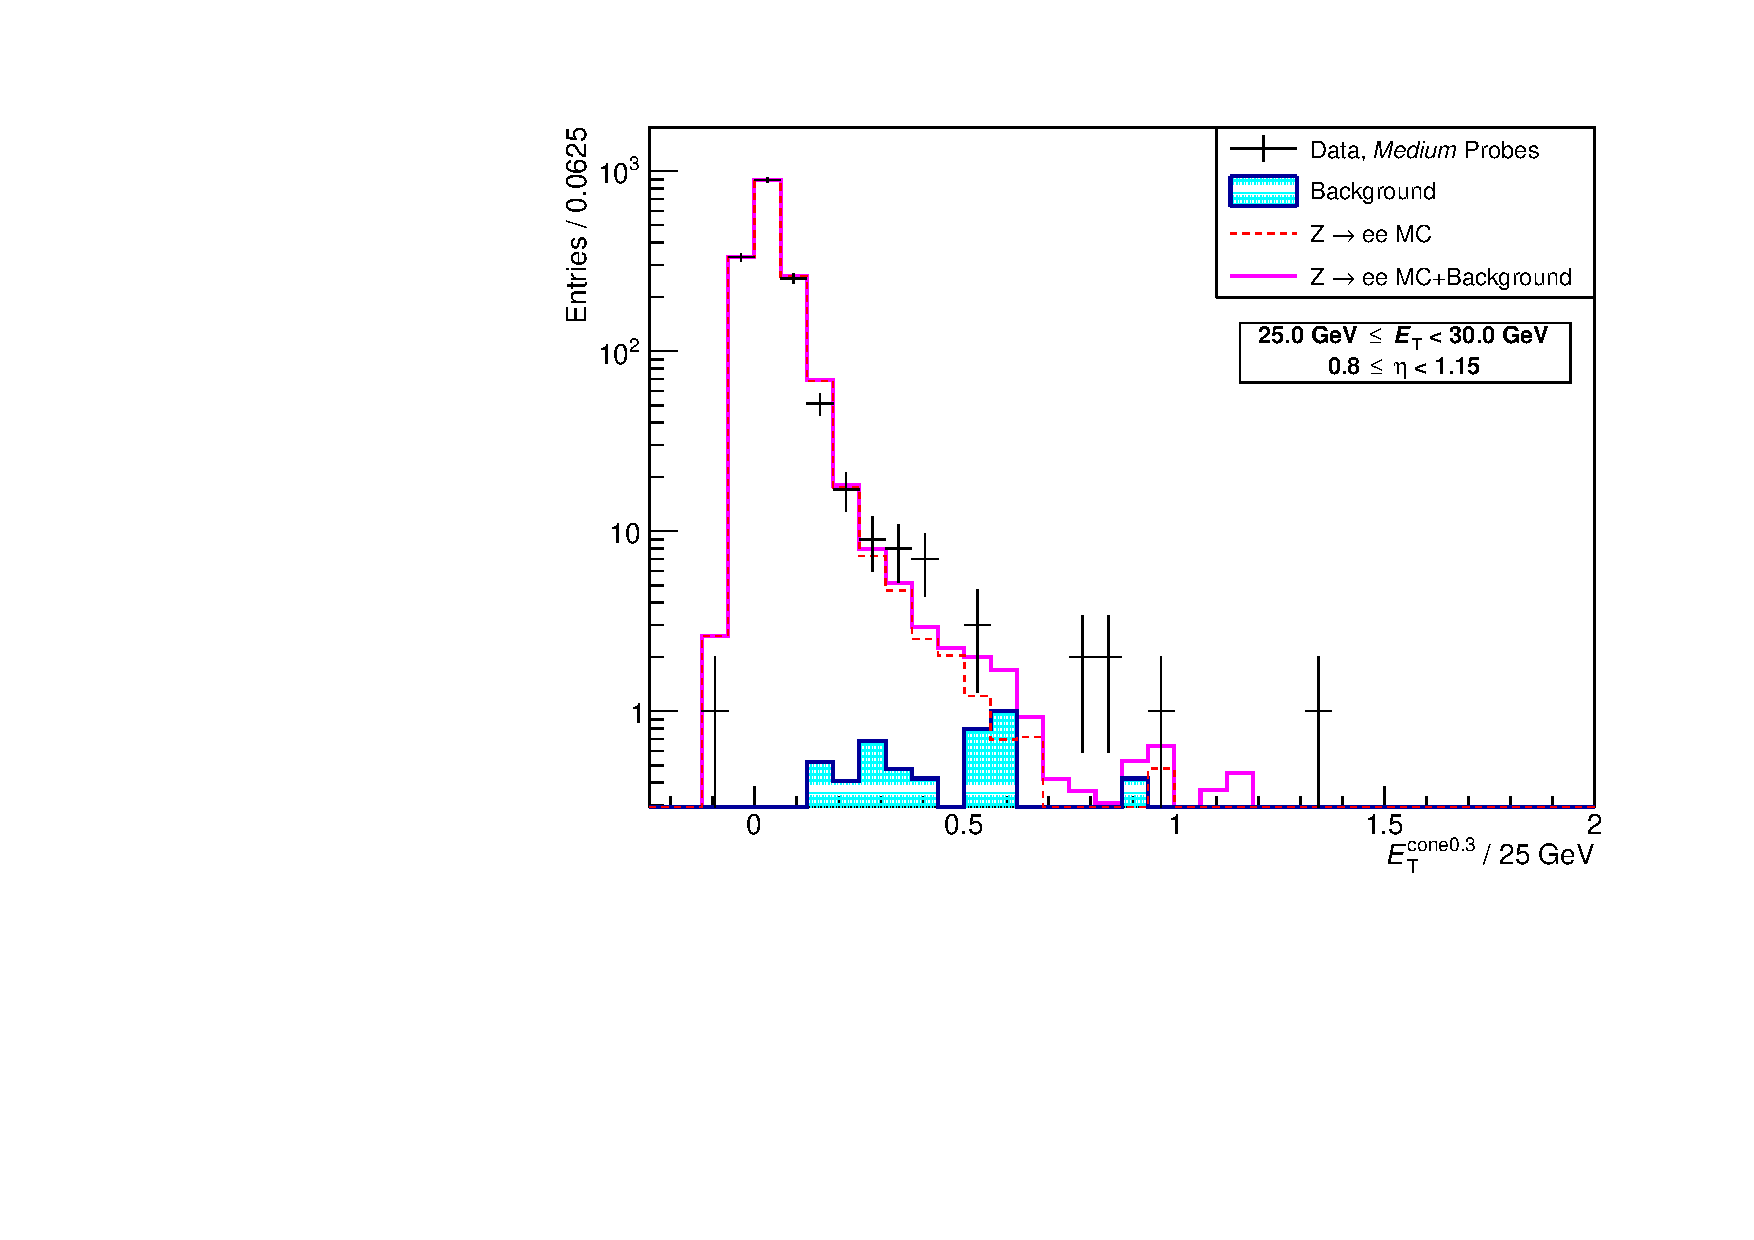
\includegraphics[width=0.48\textwidth]{Efficiencies/ID/Bkg_Num_13TeV_ZIso}
    \caption{Isolation $\et^\mathrm{cone0.3}/25 \,\GeV$ distribution of
    	probe electrons in the ZIso-method using 13 TeV $339\,\ipb$
    	low-pileup data. Left the denominator and right the numerator
    	distributions are shown, with the data as crosses, the signal \Zee
    	expectation as open line and the background estimate as cyan area
    	(template normalised at high values).}
    \label{fig:bkgfit_ziso}
    \end{figure} 
    
    The SF to be used in the analysis is constructed out of both methods. The merger of the results takes into account the high degree of correlation of the two methods and includes the following steps:
    \begin{itemize}
    	\item the final SF is defined as an arithmetic mean of the two methods over all systematic variations;
    	\item the statistical uncertainty is calculated as an average of the statistical uncertainties of the variations;
    	\item a covariance matrix is composed from all variations of the two methods and then decomposed into correlated and uncorrelated parts, providing the systematic uncertainty.
    \end{itemize}
    The combined results are presented in Fig. \ref{fig:reco_merge} and show similar results between both methods and the combination. The SFs obtained from 5 and 13 TeV data samples were not combined due to significant difference in measured efficiency.
    \begin{figure}[htbp]
    	\centering
    	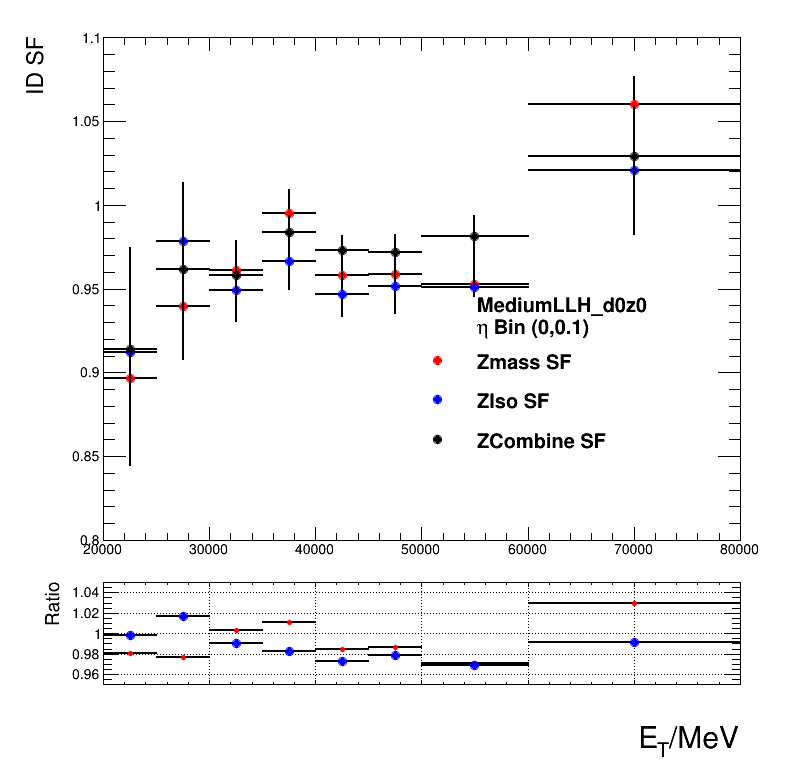
\includegraphics[width=0.35\textwidth]{Efficiencies/Reco/Merge/SF000top010}%
    	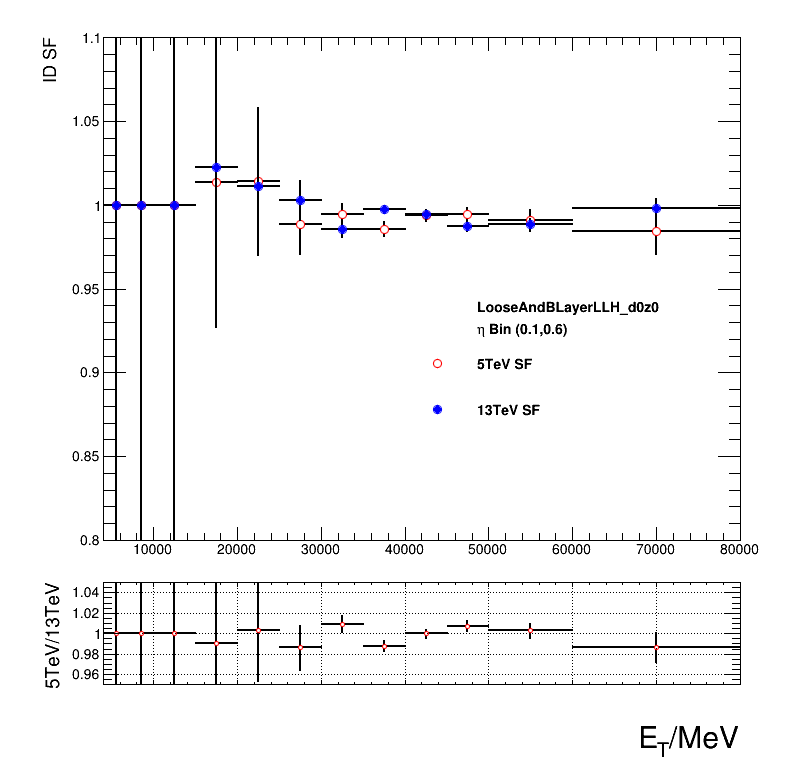
\includegraphics[width=0.35\textwidth]{Efficiencies/Reco/Merge/SFp010top060}%
    	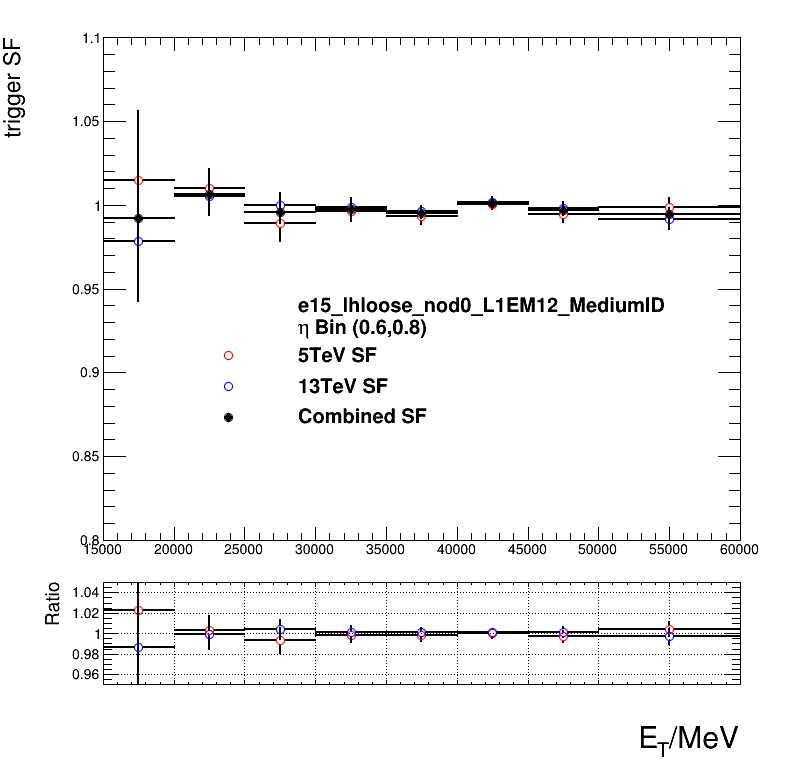
\includegraphics[width=0.35\textwidth]{Efficiencies/Reco/Merge/SFp060top080}
    	
    	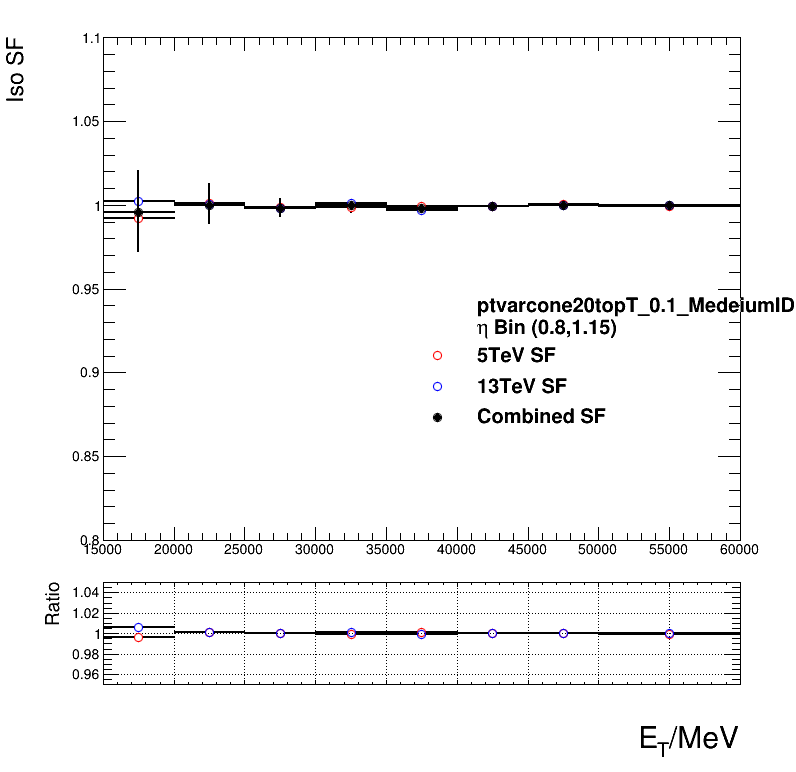
\includegraphics[width=0.35\textwidth]{Efficiencies/Reco/Merge/SFp080top115}%
    	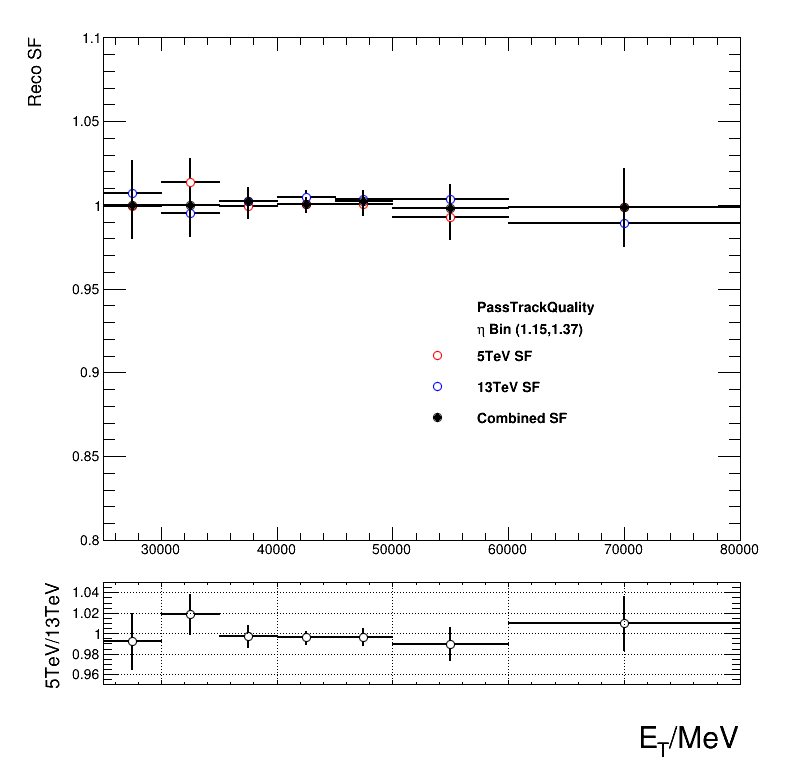
\includegraphics[width=0.35\textwidth]{Efficiencies/Reco/Merge/SFp115top137}%
    	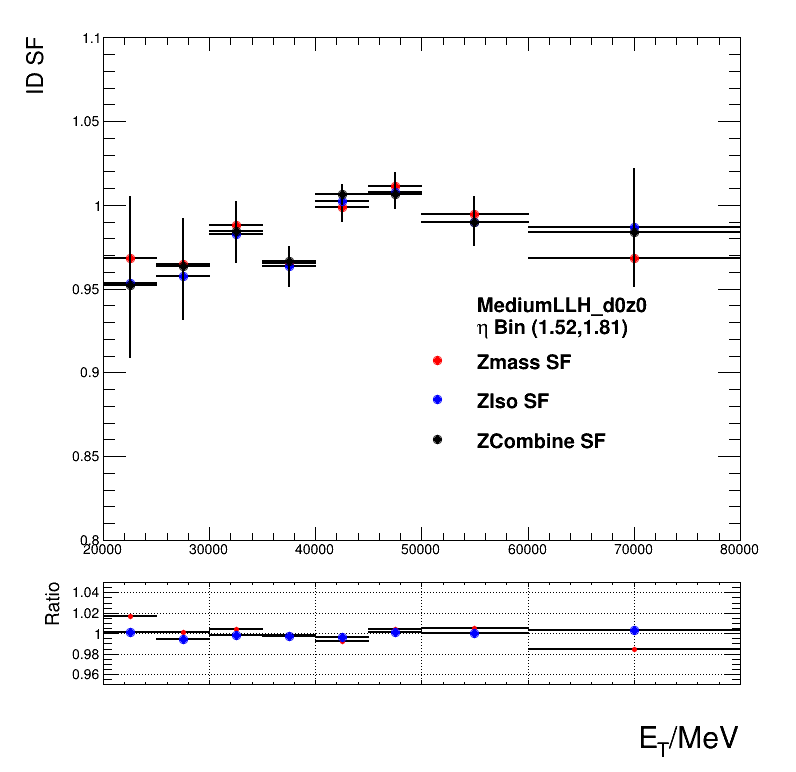
\includegraphics[width=0.35\textwidth]{Efficiencies/Reco/Merge/SFp152top181}
    	
    	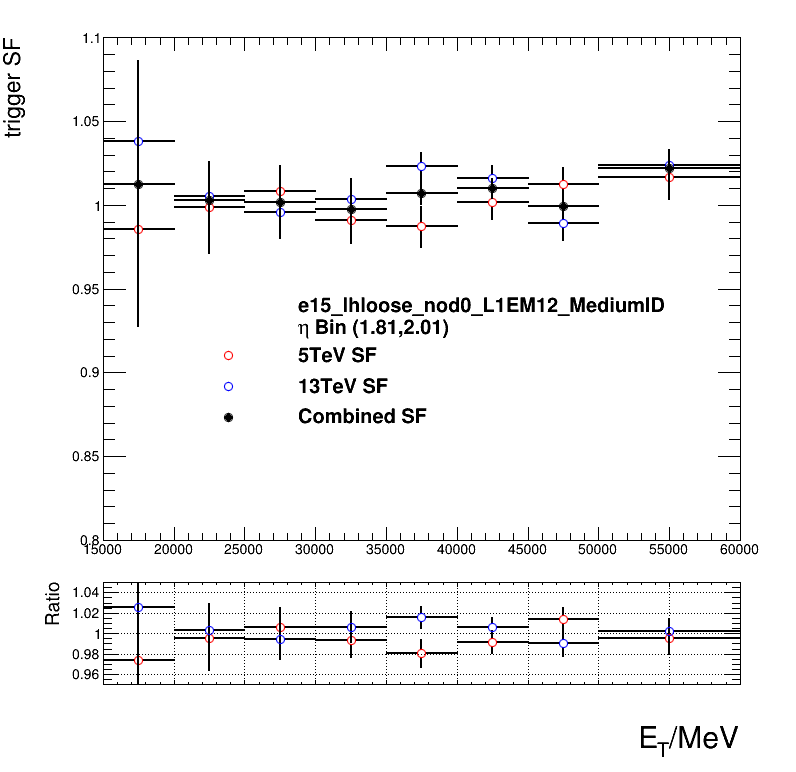
\includegraphics[width=0.35\textwidth]{Efficiencies/Reco/Merge/SFp181top201}%
    	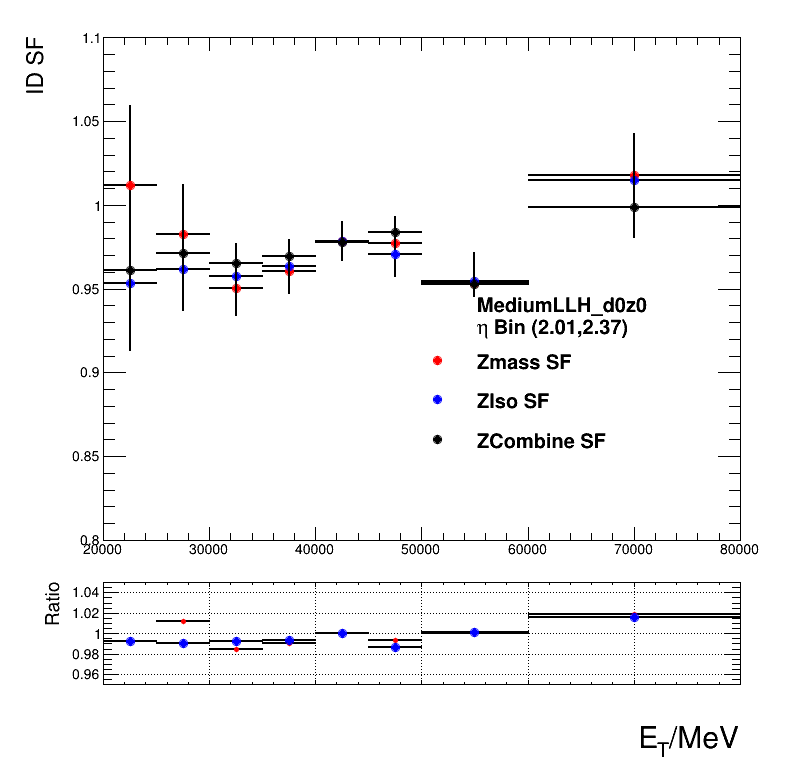
\includegraphics[width=0.35\textwidth]{Efficiencies/Reco/Merge/SFp201top237}%
    	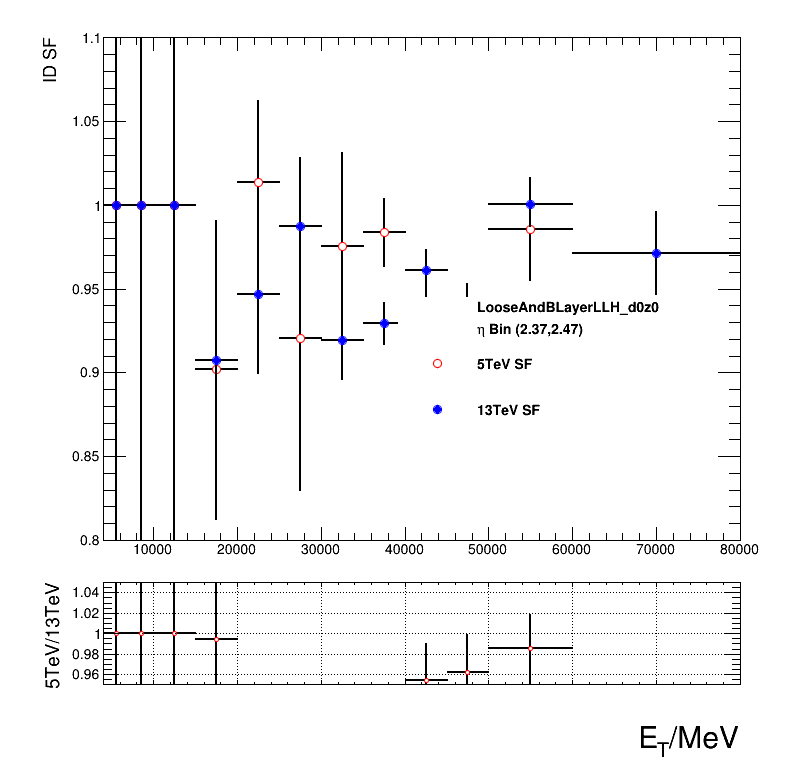
\includegraphics[width=0.35\textwidth]{Efficiencies/Reco/Merge/SFp237top247}
    	
    	\caption{Comparison of electron reconstruction SFs with 5 TeV and 13
    		TeV data as well as the 5+13 TeV combination in nine $\eta$ ranges
    		as written in the plot legend, from most central $\eta=0-0.1$ (top
    		left) to most forward $\eta=2.37-2.47$ (bottom right). The bottom panel shows the ratio
    		of 5 TeV and 13 TeV SFs. The total
    		uncertainties are shown.}  \label{fig:reco_merge}
    \end{figure}
    
    \subsubsection{Isolation efficiency}
    Electron isolation efficiency is a fraction of reconstructed and MediumLLH-identified electrons that pass a designated isolation requirement. For this analysis the isolation requirement is chosen to be $ptvarcone^{20}/p_T^e<0.1$. The results are presented in Fig. \ref{fig:iso_sf_all} and show that the efficiency is very high. The SFs for 5 and 13 TeV are not combined and used separately.
    
    \begin{figure}[htbp]
    	\centering
    	\includegraphics[width=0.47\textwidth]{Efficiencies/Iso/SF/SF25to30}
    	\includegraphics[width=0.47\textwidth]{Efficiencies/Iso/SF/SF30to35}\\
    	\includegraphics[width=0.47\textwidth]{Efficiencies/Iso/SF/SF35to40}
    	\includegraphics[width=0.47\textwidth]{Efficiencies/Iso/SF/SF40to45} \\
    	\includegraphics[width=0.47\textwidth]{Efficiencies/Iso/SF/SF45to50}
    	\includegraphics[width=0.47\textwidth]{Efficiencies/Iso/SF/SF50to60}
    	\caption{Electron isolation efficiencies (top panels) and scale
    		factors (lower panels) for the \emph{ptvarcone20}$/\pt^e < 0.1$
    		working point using 13 TeV $339\,\ipb$ low-pileup data as function
    		of $\eta$ in bins of \pt.}
    	\label{fig:iso_sf_all}
    \end{figure}
    \subsubsection{Trigger efficiency}
    During the data-taking at low pile-up the unprescaled trigger \texttt{HLT\_e15\_lhloose\_nod0\_L1EM12} was used. Thanks to the ID and isolation requirements to both tad and probe, the background is negligible for trigger efficiency measurement. Measurement results are shown in Fig. \ref{fig:trig_sf_all} and demonstrate relatively high efficiency in most of the regions. The scale factors are also very close to unity. No combination was performed between 5 and 13 TeV results.
    
    \begin{figure}[htbp]
    	\centering
    	\includegraphics[width=0.47\textwidth]{Efficiencies/Trig/SF/SF25to30}
    	\includegraphics[width=0.47\textwidth]{Efficiencies/Trig/SF/SF30to35}\\
    	\includegraphics[width=0.47\textwidth]{Efficiencies/Trig/SF/SF35to40}
    	\includegraphics[width=0.47\textwidth]{Efficiencies/Trig/SF/SF40to45} \\
    	\includegraphics[width=0.47\textwidth]{Efficiencies/Trig/SF/SF45to50}
    	\includegraphics[width=0.47\textwidth]{Efficiencies/Trig/SF/SF50to60}
    	\caption{Electron trigger efficiencies (top panels) and scale
    		factors (lower panels) for \texttt{HLT\_e15\_lhloose\_nod0\_L1EM12}
    		using 13 TeV $339\,\ipb$ low-pileup data as function
    		of $\eta$ in bins of \pt.}
    	\label{fig:trig_sf_all}
    \end{figure}
    
    
    \subsection{SF uncertainties propagation}
    The main source of uncertainty for the measurement of the SFs is coming from the background. The uncertainties are estimated by varying the parameters that contribute to background suppression. These parameters include:
    \begin{itemize}
    	\item The Zmass window technique is used by identification, isolation and trigger efficiencies measurement. The size of the Zmass window was varied in a range of 10, 15 and 20 GeV. This variation dominates at higher values of $p_T$.
    	\item Tag identification and isolation criteria were varied between Medium ID + calorimeter isolation, TightLLH and Tight ID + calorimeter isolation.
    	\item Background template has a major influence on the estimate of signal contamination, especially at $p_T<30$ GeV. In addition to the nominal rage of template extraction in $120 < m_{ee} < 250$ the templates are also normalized using the region of $60 < m_{ee} < 70$ GeV.
    	\item Side band range is varied for reconstruction efficiency measurement. 
    	\item Isolation criteria are varied in the measurement of ID efficiency: $E_T^{cone0.3}/25\gev$ is varied between 0.4, 0.5 and 0.6, also a larger cone isolation around the probe electron was used - $E_T^{cone0.4}/25\gev$.
    \end{itemize}
    
    Figure \ref{fig:all_uncertainty_tp} shows the total relative uncertainties of the electron scale factors at 13 TeV in different $\eta$ bins. Contributions from reconstruction and identification are the dominant ones. The uncertainties are propagated to the observables using the co-called Full correlation model (see Ref. \cite{topoclust_2019}). The idea of the method is to split the sources of SF uncertainty into uncorrelated and correlated sources. Uncorrelated sources are of statistical nature and mostly related to the number of \Zee pairs in different bins if $p_T$ and $\eta$ used for SF extraction. Correlated sources of systematic uncertainty arise from the flaws of background subtraction. In the Full correlation model includes about 10 sources of systematic uncertainty and around 200 $p_T\times\eta$ bins as sources of statistical uncertainty and allows to propagate these uncertainties to the observables. Figures \ref{fig:total_sys_13_medium} and \ref{fig:total_sys_5_medium} contain the results of error propagation for 13 and 5 \tev{} respectively. Again, identification and reconstruction uncertainties have the largest contribution to the total SF uncertainty. 
    
    \begin{figure}[htbp]
    	\centering
    	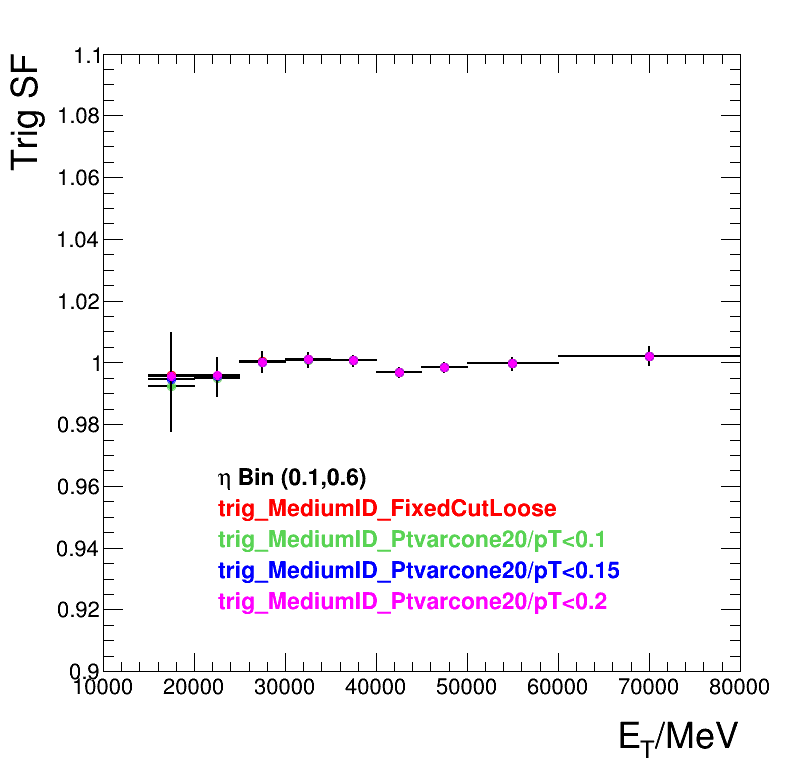
\includegraphics[width=0.32\textwidth]{Efficiencies/Uncer/Total/p010_p060}
    	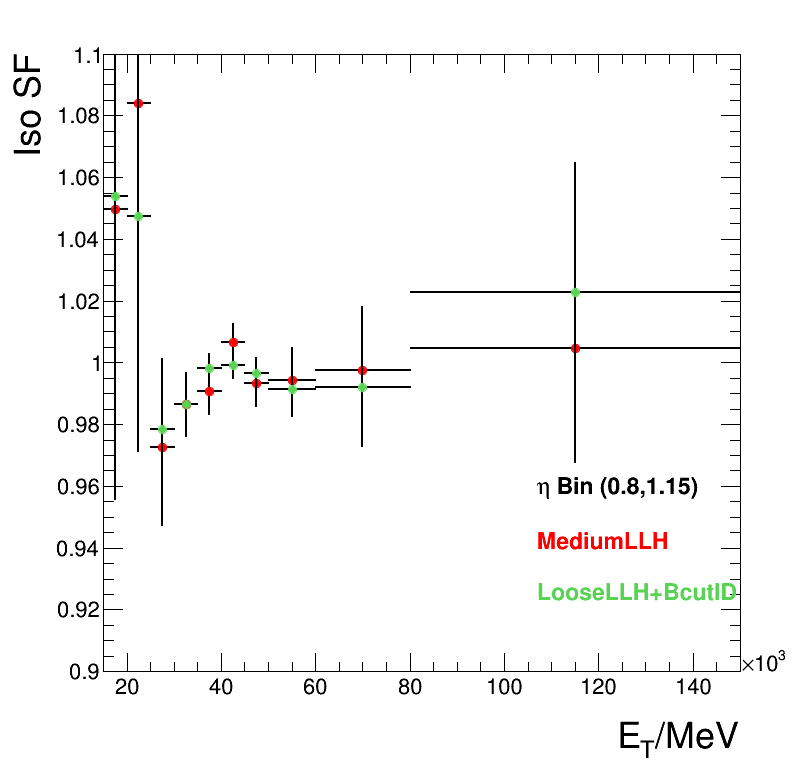
\includegraphics[width=0.32\textwidth]{Efficiencies/Uncer/Total/p080_p115}
    	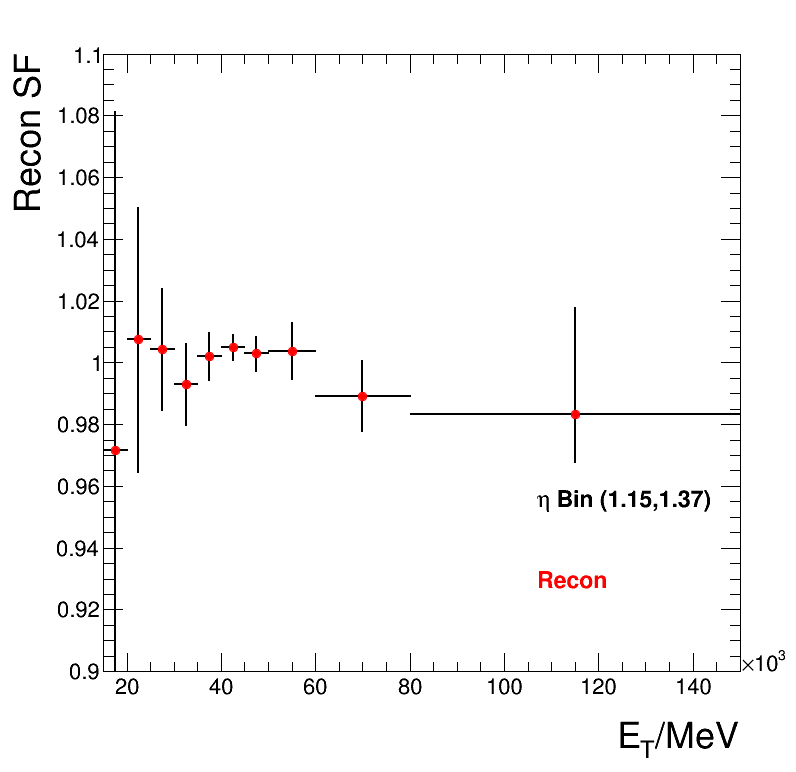
\includegraphics[width=0.32\textwidth]{Efficiencies/Uncer/Total/p115_p137} \\
    	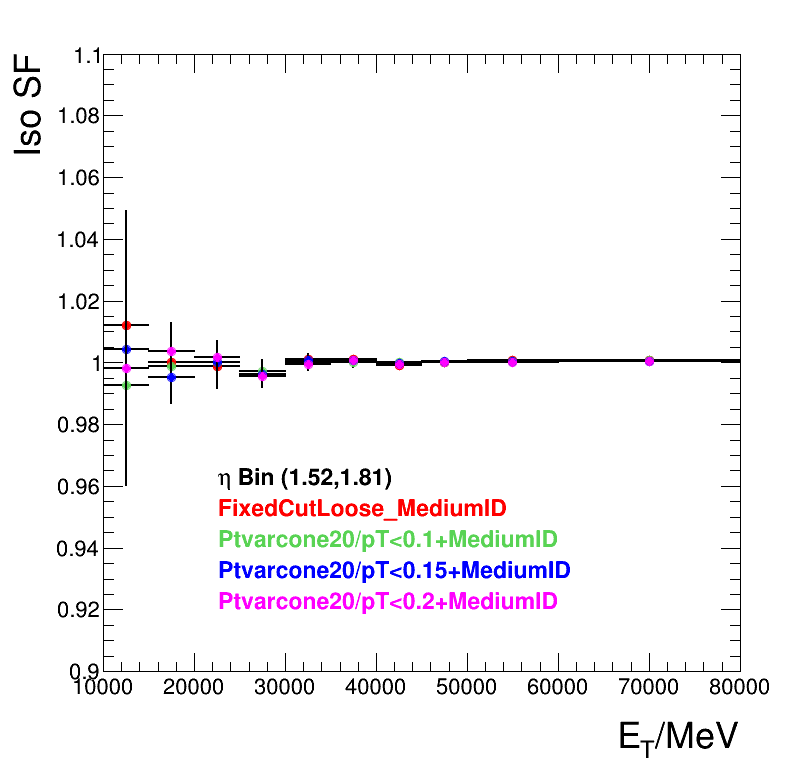
\includegraphics[width=0.32\textwidth]{Efficiencies/Uncer/Total/p152_p181}
    	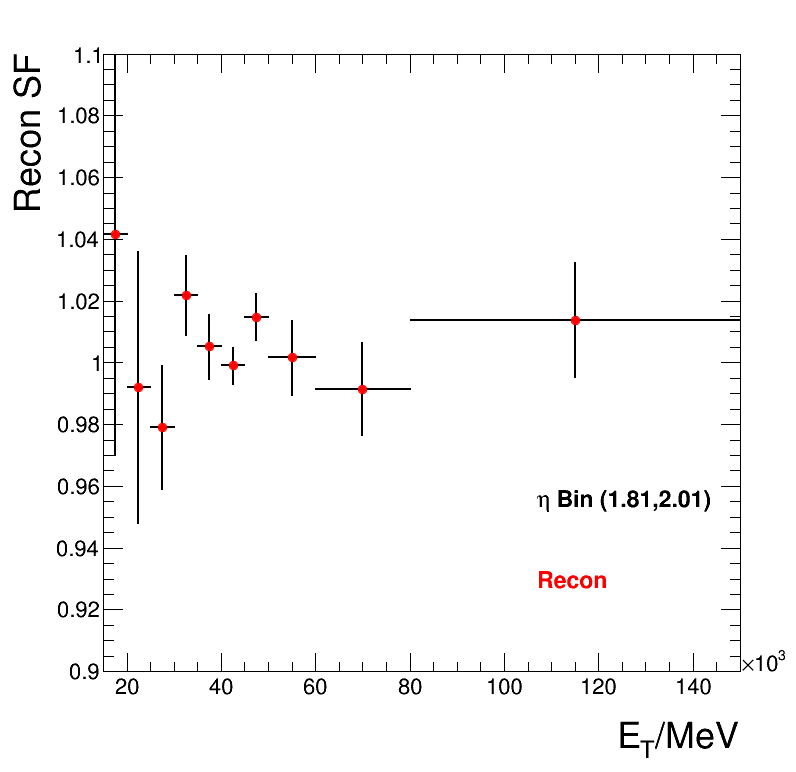
\includegraphics[width=0.32\textwidth]{Efficiencies/Uncer/Total/p181_p201}
    	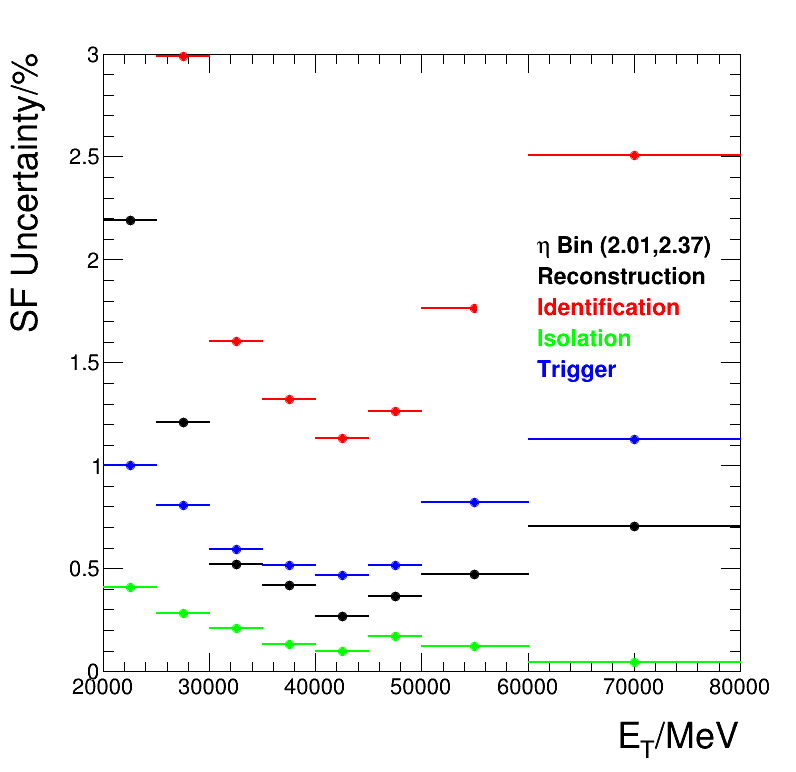
\includegraphics[width=0.32\textwidth]{Efficiencies/Uncer/Total/p201_p237} \\
    	\caption{Total relative uncertainties of electron scale factors at 13 TeV measured with tag-and-probe method}
    	\label{fig:all_uncertainty_tp}
    \end{figure}
    
    \begin{figure}[htbp]
    	\begin{center}
    		\includegraphics[width=0.48\textwidth]{Efficiencies/Uncer/13TeVMedium_extra_new/syspt}
    		\includegraphics[width=0.48\textwidth]{Efficiencies/Uncer/13TeVMedium_extra_new/syseta}
    		\includegraphics[width=0.48\textwidth]{Efficiencies/Uncer/13TeVMedium_extra_new/sys_met}
    		\includegraphics[width=0.48\textwidth]{Efficiencies/Uncer/13TeVMedium_extra_new/sys_mT}
    		\includegraphics[width=0.48\textwidth]{Efficiencies/Uncer/13TeVMedium_extra_new/boson_pT}
    		\caption{Contributions to the electron uncertainties related to
    			efficiency SF (reconstruction, identification, isolation and
    			trigger) in a $W^{+}\rightarrow e^{+}\nu$ selection at 13 TeV as
    			function of typical kinematic variables.}
    		\label{fig:total_sys_13_medium}
    	\end{center}
    \end{figure}
    
    
    \begin{figure}[htbp]
    	\begin{center}
    		\includegraphics[width=0.48\textwidth]{Efficiencies/Uncer/5TeVMedium_extra_new/syspt}
    		\includegraphics[width=0.48\textwidth]{Efficiencies/Uncer/5TeVMedium_extra_new/syseta}
    		\includegraphics[width=0.48\textwidth]{Efficiencies/Uncer/5TeVMedium_extra_new/sys_met}
    		\includegraphics[width=0.48\textwidth]{Efficiencies/Uncer/5TeVMedium_extra_new/sys_mT}
    		\includegraphics[width=0.48\textwidth]{Efficiencies/Uncer/5TeVMedium_extra_new/boson_pT}
    		\caption{Contributions to the electron uncertainties related to
    			efficiency SF (reconstruction, identification, isolation and
    			trigger) in a $W^{+}\rightarrow e^{+}\nu$ selection at 5 TeV as
    			function of typical kinematic variables.}
    		\label{fig:total_sys_5_medium}
    	\end{center}
    \end{figure}
    \clearpage
    
    \section{Muon corrections}
	Muon corrections are in many aspects similar to the electron corrections described in the previous section. Calibrations are used in order to match the data and MC simulation 
    \subsection{Muon momentum calibration}
	The muon momentum calibration comprises corrections to the momentum scale and resolution. At first the \gls{id} and \gls{ms} tracks are reconstructed and corrected separately, and then the two corrections are propagated to correct the CB muon tracks. Low energy muons with $5<p_T<30$ GeV are calibrated using the $J/psi\rightarrow\mu\mu$ resonance, while in higher energy region of $22<p_T<300$ GeV the $Z \rightarrow\mu\mu$ resonance is used. The statistical uncertainties are directly linked to the number of Z and $J/psi$ candidates in the data samples:
	\begin{itemize}
			\item{5.02~\TeV\ data (2017, period M): 660k $J/\psi$ candidates, 75k $Z$ candidates}
			\item{13~\TeV\ data (2017, period N): 1.1M $J/\psi$ candidates, 100k $Z$ candidates}
			\item{13~\TeV\ data (2018, periods G4 and J): 1.5M $J/\psi$ candidates, 130k $Z$ candidates}
	\end{itemize}
	The Z and $J/psi$ peaks are fitted with a function that is a sum of a Crystal Ball function (that fits the mass peak), a Gaussian (that accounts for effects like multiple scattering) and an exponential that fits the backgrounds. The examples of such fits are presented at Fig. \ref{fig:calib-fits}.
	
	\begin{figure}[htb!]
		\begin{center}
			\includegraphics[width=0.49\textwidth]{calibration/13TeV_2017/example-fit-Jpsi.pdf}
			\includegraphics[width=0.49\textwidth]{calibration/13TeV_2017/example-fit.pdf}
			\caption{Example fits to $J/\psi \to \mu\mu$~(left) and \Zmm~(right) mass peaks for pairs with leading muon pseudorapidity in the range $-0.62<\eta<-0.52$ in low-pile-up 2017 13~\TeV\ data.}
			\label{fig:calib-fits}
		\end{center}
	\end{figure}

	The measured correction parameters for Z and $J/psi$ peaks for 5 and 13 TeV are presented in Figures \ref{fig:calib-Jpsi-5TeV}, \ref{fig:calib-Jpsi-13TeV}, \ref{fig:calib-Z-5TeV} and \ref{fig:calib-Z-13TeV}.
	
	\begin{figure}[htb!]
		\begin{center}
			\includegraphics[width=0.49\textwidth]{calibration/5TeV/Jpsi_ID_Scale_Eta1.pdf}
			\includegraphics[width=0.49\textwidth]{calibration/5TeV/Jpsi_ID_Resolution_Eta0.pdf}\\
			\includegraphics[width=0.49\textwidth]{calibration/5TeV/Jpsi_ME_Scale_Eta1.pdf}
			\includegraphics[width=0.49\textwidth]{calibration/5TeV/Jpsi_ME_Resolution_Eta0.pdf}\\
			\includegraphics[width=0.49\textwidth]{calibration/5TeV/Jpsi_CB_Scale_Eta1.pdf}
			\includegraphics[width=0.49\textwidth]{calibration/5TeV/Jpsi_CB_Resolution_Eta0.pdf}
			\caption{Mean~(left) and width~(right) of the $J/\psi \to \mu\mu$ mass peak as a function of the leading muon $\eta$ in 5.02~\TeV\ data and MC. The mean and width are extracted from Crystal Ball components of the fits. In case of the simulation, both the uncorrected~(dashed histogram) and corrected parameters~(solid histogram) are shown. The fit results are presented for mass peaks constructed using kinematics of the muon ID tracks~(top), ME tracks~(middle) or CB tracks~(bottom). The bottom panels in each plot show the data/MC ratio for uncorrected~(dashed histogram) and corrected simulation~(points).}
			\label{fig:calib-Jpsi-5TeV}
		\end{center}
	\end{figure}
	
	\begin{figure}[htb!]
		\begin{center}
			\includegraphics[width=0.49\textwidth]{calibration/13TeV_2017/Jpsi_ID_Scale_Eta1.pdf}
			\includegraphics[width=0.49\textwidth]{calibration/13TeV_2017/Jpsi_ID_Resolution_Eta0.pdf}\\
			\includegraphics[width=0.49\textwidth]{calibration/13TeV_2017/Jpsi_ME_Scale_Eta1.pdf}
			\includegraphics[width=0.49\textwidth]{calibration/13TeV_2017/Jpsi_ME_Resolution_Eta0.pdf}\\
			\includegraphics[width=0.49\textwidth]{calibration/13TeV_2017/Jpsi_CB_Scale_Eta1.pdf}
			\includegraphics[width=0.49\textwidth]{calibration/13TeV_2017/Jpsi_CB_Resolution_Eta0.pdf}
			\caption{Mean~(left) and width~(right) of the $J/\psi \to \mu\mu$ mass peak as a function of the leading muon $\eta$ in 2017 13~\TeV\ data and MC at low pile-up. The mean and width are extracted from Crystal Ball components of the fits. In case of the simulation, both the uncorrected~(dashed histogram) and corrected parameters~(solid histogram) are shown. The fit results are presented for mass peaks constructed using kinematics of the muon ID tracks~(top), ME tracks~(middle) or CB tracks~(bottom). The bottom panels in each plot show the data/MC ratio for uncorrected~(dashed histogram) and corrected simulation~(points).}
			\label{fig:calib-Jpsi-13TeV}
		\end{center}
	\end{figure}

	\begin{figure}[htb!]
		\begin{center}
			\includegraphics[width=0.49\textwidth]{calibration/5TeV/Z_ID_Scale_Eta1.pdf}
			\includegraphics[width=0.49\textwidth]{calibration/5TeV/Z_ID_Resolution_Eta0.pdf}\\
			\includegraphics[width=0.49\textwidth]{calibration/5TeV/Z_ME_Scale_Eta1.pdf}
			\includegraphics[width=0.49\textwidth]{calibration/5TeV/Z_ME_Resolution_Eta0.pdf}\\
			\includegraphics[width=0.49\textwidth]{calibration/5TeV/Z_CB_Scale_Eta1.pdf}
			\includegraphics[width=0.49\textwidth]{calibration/5TeV/Z_CB_Resolution_Eta0.pdf}
			\caption{Mean~(left) and width~(right) of the \Zmm\ mass peak as a function of the leading muon $\eta$ in 5.02~\TeV\ data and MC. The mean and width are extracted from Crystal Ball components of the fits. In case of the simulation, both the uncorrected~(dashed histogram) and corrected parameters~(solid histogram) are shown. The fit results are presented for mass peaks constructed using kinematics of the muon ID tracks~(top), ME tracks~(middle) or CB tracks~(bottom). The bottom panels in each plot show the data/MC ratio for uncorrected~(dashed histogram) and corrected simulation~(points).}
			\label{fig:calib-Z-5TeV}
		\end{center}
	\end{figure}
	
	\begin{figure}[htb!]
		\begin{center}
			\includegraphics[width=0.49\textwidth]{calibration/13TeV_2017/Z_ID_Scale_Eta1.pdf}
			\includegraphics[width=0.49\textwidth]{calibration/13TeV_2017/Z_ID_Resolution_Eta0.pdf}\\
			\includegraphics[width=0.49\textwidth]{calibration/13TeV_2017/Z_ME_Scale_Eta1.pdf}
			\includegraphics[width=0.49\textwidth]{calibration/13TeV_2017/Z_ME_Resolution_Eta0.pdf}\\
			\includegraphics[width=0.49\textwidth]{calibration/13TeV_2017/Z_CB_Scale_Eta1.pdf}
			\includegraphics[width=0.49\textwidth]{calibration/13TeV_2017/Z_CB_Resolution_Eta0.pdf}
			\caption{Mean~(left) and width~(right) of the \Zmm\ mass peak as a function of the leading muon $\eta$ in 2017 13~\TeV\ data and MC at low pile-up. The mean and width are extracted from Crystal Ball components of the fits. In case of the simulation, both the uncorrected~(dashed histogram) and corrected parameters~(solid histogram) are shown. The fit results are presented for mass peaks constructed using kinematics of the muon ID tracks~(top), ME tracks~(middle) or CB tracks~(bottom). The bottom panels in each plot show the data/MC ratio for uncorrected~(dashed histogram) and corrected simulation~(points).}
			\label{fig:calib-Z-13TeV}
		\end{center}
	\end{figure}
	\subsection{Correction for charge-dependent momentum bias}
    Misalignment in \gls{id}, \gls{ms} or between the two systems can lead to a charge-dependent bias (also called \textit{sagitta bias}) of muon reconstructed momentum. Its effect can be parametrized as follows:
    \begin{equation}
    	p_T^{meas}=\frac{p_T^{reco}}{1+q\dot \delta_{sagitta}\dot p_T^{reco}},
    \end{equation}
    where $p_T^{meas}$ is the measured momentum that contains a bias, $p_T^{reco}$ is the unbiased reconstructed momentum and the bias to be corrected is denoted as $\delta_{sagitta}$.\\
    The sagitta correction is obtained as a function of $\eta$. There exist three methods of sagitta bias determination:
    \begin{itemize}
    	\item The ID alignment and momentum measurement can be tested with electrons which have additional information from the charge-independent calorimeter. Using \Zee and/or \Wenu events it is possible to determine the charge bias of an electron track:
    	\begin{equation}
    		\delta_{sagitta}=\frac{<E/p_{track}>^+-<E/p_{track}>^-}{2<p^{calo}_T>},
    	\end{equation}
    	where $p_{track}$ is the momentum measured in the \gls{id}, E is the energy measured in the \gls{emc}, from which we can get the $p^{calo}_T=E\dot \sin{\theta}$ transverse momentum. The $<>$ brackets denote the averaging in $\eta$ bins. 
    	\item The $p_T(\mu)$ method is used by \gls{mcp} and alignment groups in high-$\mu$ data compares the muons and anti-muons spectra in \Zmm events.
    	\item The Z-mass method uses the Z mass peak. This is the main method used my \gls{mcp} and alignment groups, the results are denoted as $M_{\mu\mu}\_MCP$ and $M_{\mu\mu}\_Align$ on the plots (see \cite{muon_align}). The sagitta bias is calculated iteratively minimizing the difference between the reconstructed and expected position of the \Zmm mass peak position.
    \end{itemize}
	The results of these methods are presented in Fig. \ref{fig:allsagitta}. The sagitta bias in low-pile-up data was found to be 10 times higher than in the MC simulation. Further results in the measurement rely on the following method: the differences between the data and MC are averaged over $\eta$ using a fit, and also introduce a global offset. The results are shown in Fig. \ref{fig:sagittacorrection}.
	
	
    \begin{figure}[p]
    	\begin{center}
    		\includegraphics[width=0.48\textwidth]{sagitta/data_sagitta}
    		\includegraphics[width=0.48\textwidth]{sagitta/MC_sagitta}
    		\caption{Sagitta bias corrections derived for 2017 low-pile-up data (left)
    			and simulation (right) at $\sqrt{s} = 13$~\TeV. The
    			corrections are evaluated with two $Z$-mass methods
    			(``$M\mu\mu$\_MCP'' and ``$M\mu\mu$\_Align''),
    			the $E/p$ method applied to \Wenu (``Wenv\_E/p'') and \Zee (``Zee\_E/p'')
    			events, and the $\pt(\mu)$ method, all of which are discussed in the text.
    			The top plot shows the data
    			results, where with clear $\eta$-dependent and overall biases
    			are observed. The bottom plot shows MC, where a bias smaller by a factor of at least 10,
    			with the exception of the electron $E/p$ method.}
    		\label{fig:allsagitta}
    	\end{center}
    \end{figure}
	

\begin{figure}[htb!]
	\begin{center}
		\includegraphics[width=0.49\textwidth]{sagitta/correction}
		\caption{Sagitta bias correction based on 2017 low-pile-up
			data at $\sqrt{s} = 13$~\TeV. The statistical
			uncertainty (combined from uncertainties of the
			$\eta$-dependent correction and the global offset
			correction) is represented by error bars.}
		\label{fig:sagittacorrection}
	\end{center}
\end{figure}
\clearpage

    \subsection{Muon efficiency measurements}
    Just like in the case of electrons, muons have to pass a number of quality criteria in order to be used in the analysis:
    \begin{itemize}
    	\item Reconstruction and identification: the muon is successfully reconstructed and its \gls{id} and \gls{ms} tracks as well as \gls{emc} deposit are matched. The \textit{medium} identification criterion is adopted for the low-$\mu$ analysis. Only CB and ME muons with loose requirements between the tracks from \gls{id} and \gls{ms} are used. The value of $q/p$ significance is required to be $<7$. 
    	\item Isolation: \textit{LowMuWZPtvarcone20} selection was used, it has the track isolation requirement of $p_T^{varcone20}/p_T<0.1$. 
    	\item Trigger: the muons were required to mass the $HLT\_mu14$ trigger.
    	\item \gls{ttva} includes requirement for the muon track to match the primary vertex. The muon objects are required to pass $|z_0|\sin{\theta}<0.5$ mm and $d_0/\sigma(d_0)<3$ requirements.
    \end{itemize}
	Just like in the case of electrons, possible discrepancies between the data and MC are corrected using the scale factors, which are in turn measured using the tag-and-probe method described in \cite{Koehler:2665704}. The product of the scale factors define the event weight: 
	\begin{equation*}
	W_{event}^{W\rightarrow e\nu}=SF_{reco/ID} \dot SF_{trig} \dot SF_{TTVA} \dot SF_{iso}.
	\end{equation*}
	All muon efficiencies and scale factors used in current analysis are measured in-situ using the low-$\mu$ datasets at 5 and 13 TeV by the \gls{mcp} group. The results for their measurements are presented in Figures 
	
	\begin{figure}
		\centering
		\includegraphics[width=0.495\textwidth]{lowMuComp_2017_13_reco/Eff_EtaVar_Aux_EtaVar_IDProbesWithMS_AllPt10_MediumMuons}%
		\includegraphics[width=0.495\textwidth]{lowMuComp_2017_13_reco/Eff_PtWVar_Aux_PtWVar_IDProbesWithMS_AllPt10_MediumMuons}
		\includegraphics[width=0.495\textwidth]{lowMuComp_2017_5_reco/Eff_EtaVar_Aux_EtaVar_IDProbesWithMS_AllPt10_MediumMuons}%
	\includegraphics[width=0.495\textwidth]{lowMuComp_2017_5_reco/Eff_PtWVar_Aux_PtWVar_IDProbesWithMS_AllPt10_MediumMuons}
		\includegraphics[width=0.495\textwidth]{lowMuComp_2018_reco/Eff_EtaVar_Aux_EtaVar_IDProbesWithMS_AllPt10_MediumMuons}%
	\includegraphics[width=0.495\textwidth]{lowMuComp_2018_reco/Eff_PtWVar_Aux_PtWVar_IDProbesWithMS_AllPt10_MediumMuons}
	
		\caption{Comparison of reconstruction efficiencies for Medium muons
			using the low-$\mu$ runs of 2017 and 2018 at a centre-of-mass energy of
			$\sqrt{s}=13\,$TeV and $\sqrt{s}=5\,$TeV. Efficiencies are
			shown as a function of muon $\eta, \pT$. Red (orange) points correspond to low-$\mu$ data (MC),
			while the black (blue) points are high-$\mu$ data (MC). The bottom
			panels show the data/MC ratio for the low-$\mu$ (orange) and
			high-$\mu$ (blue) sets with statistical and total
			uncertainties.}\label{app:fig:lowMu2}
	\end{figure}
	
	\begin{figure}  \centering
		\includegraphics[width=0.49\textwidth]{lowMuComp_201718_ttva/Eff_Eta1D22_Aux_Eta1D22_LooseProbes_noProbeIP_All_IPCutEff}%
		\includegraphics[width=0.49\textwidth]{lowMuComp_201718_ttva/Eff_Pt1D20_Aux_Pt1D20_LooseProbes_noProbeIP_All_IPCutEff}
		\includegraphics[width=0.49\textwidth]{lowMuComp_201718_ttva/Eff_Mu10_Aux_Mu10_LooseProbes_noProbeIP_All_IPCutEff}%
		\includegraphics[width=0.49\textwidth]{lowMuComp_2017_5_ttva/Eff_Eta_Aux_Eta_LooseProbes_noProbeIP_All_IPCutEff}
		\includegraphics[width=0.49\textwidth]{lowMuComp_2017_5_ttva/Eff_PtNoVar_Aux_PtNoVar_LooseProbes_noProbeIP_All_IPCutEff}%
		\includegraphics[width=0.49\textwidth]{lowMuComp_2017_5_ttva/Eff_Mu10_Aux_Mu10_LooseProbes_noProbeIP_All_IPCutEff}
	
		\caption{Comparison of TTVA efficiencies for Medium muons using the
			low-$\mu$ runs of 2017+18 at $\sqrt{s}=13$~\TeV{} (top row) and
			low-$\mu$ runs of 2017 at $\sqrt{s}=5$~\TeV{} (lower row).
			The low-$\mu$ results compared to a high-$\mu$ data set as specified in the plot legend.
			Efficiencies are shown as function of muon $\eta$ (left) and
			$\pT$ (middle) and the mean number of interactions $<\mu>$
			(right). Red (orange) points correspond to low-$\mu$ data (MC),
			while the black (blue) points are high-$\mu$ data (MC). The bottom
			panels show the data/MC ratio for the low-$\mu$ (orange) and
			high-$\mu$ (blue) sets with statistical and total
			uncertainties.}\label{app:fig:ttva-lowMu1}
	\end{figure}
	\begin{figure}
		\centering
		\includegraphics[width=0.49\textwidth]{trigger/13TeVEffs_medium_periodJ_Eff_BarrelEtaCoarse_LooseProbes_noProbeIP_All_HLT_mu14_noDDBkg}
		\includegraphics[width=0.49\textwidth]{trigger/13TeVEffs_medium_periodJ_Eff_Pt_LooseProbes_noProbeIP_All_HLT_mu14_noDDBkg}
		\includegraphics[width=0.49\textwidth]{trigger/13TeVEffs_medium_periodN_Eff_BarrelEtaCoarse_LooseProbes_noProbeIP_All_HLT_mu14_noDDBkg}
		\includegraphics[width=0.49\textwidth]{trigger/13TeVEffs_medium_periodN_Eff_Pt_LooseProbes_noProbeIP_All_HLT_mu14_noDDBkg}
		\includegraphics[width=0.49\textwidth]{trigger/5TeVEffs_medium_Eff_BarrelEtaCoarse_LooseProbes_noProbeIP_All_HLT_mu14_noDDBkg}
		\includegraphics[width=0.49\textwidth]{trigger/5TeVEffs_medium_Eff_Pt_LooseProbes_noProbeIP_All_HLT_mu14_noDDBkg}
		
		\caption{1D trigger efficiency and systematic uncertainty in data and MC, 5 and 13 TeV from 2017 and 2018 for probes from the eta barrel region and inclusive $\phi$, $\pt$ distributions. Trigger sectors in the barrel and endcap regions are different, only the barrel trigger is shown here. The bin edges correspond to physical edges of the trigger sectors. } \label{trig:1d2018}
	\end{figure}

	\begin{figure}[pt]
		\begin{center}
			\includegraphics[width=0.49\textwidth]{isolation/13TeV_2018/Eff_Eta_IsoSFNom_All_IsoFixedCutLoose.pdf}
			\includegraphics[width=0.49\textwidth]{isolation/13TeV_2018/Eff_PtLimited_IsoSFNom_All_IsoFixedCutLoose.pdf}\\
			\includegraphics[width=0.49\textwidth]{isolation/13TeV_2017/Eff_Eta_IsoSFNom_All_IsoLowMuWZPtvarcone30.pdf}
			\includegraphics[width=0.49\textwidth]{isolation/13TeV_2017/Eff_PtLimited_IsoSFNom_All_IsoLowMuWZPtvarcone30.pdf}\\
			\includegraphics[width=0.49\textwidth]{isolation/5TeV/Eff_Eta_IsoSFNom_All_IsoLowMuWZPtvarcone20.pdf}
			\includegraphics[width=0.49\textwidth]{isolation/5TeV/Eff_PtLimited_IsoSFNom_All_IsoLowMuWZPtvarcone20.pdf}
			\caption{Efficiencies for Ptvarcone20 isolation selections measured in 2017 and 2018 data and MC 13~\TeV\  and 5~\TeV\ as a function of muon $\eta$~(left) and \pt~(right). The bottom panels show the data/MC scale factors with statistical uncertainties represented by blue boxes, while a sum in quadrature of statistical and systematic uncertainties is represented by orange boxes.}
			\label{fig:iso-sf-13TeV-2018}
		\end{center}
	\end{figure}
	
	\clearpage

     \section{Hadronic recoil calibration}
     The study of the W boson kinematics by its leptonic decay products $W^{\pm}\rightarrow l^{\pm} \nu$ is complicated first of all due to the escaping neutrino that carries away substantial information. However, the W boson transverse momentum can still be measured. As it was shown in Chapter 5, the largest part of the W boson $p_T$ is coming from the initial state radiation. The energy of the created parton shower can be measured:
	\begin{equation}
	\vec{\ptv}=\vec{\pt}^{\ell}+\vec{\pt}^{\nu} = -\sum_{i=\mathrm{ISR}\, q,g} \vec{\pt}_i = -\vec{\ut}\;,
	\end{equation}
	where $\vec{\ptv}$, $\vec{\pt}^{\ell}$ and $\vec{\pt}^{\nu}$ are the transverse momenta of the vector boson, lepton and neutrino respectively. The vector sum of all the partons from the ISR is called the \textit{hadronic recoil}: $\sum_{i=\mathrm{ISR}\, q,g} \vec{\pt}_i = \vec{\ut}$. Then the missing transverse momentum $\vec{\met} $ of the escaping neutrino can be measured as:
	\begin{equation}\label{eq:METandNeutrino}
	\vec{\met} = \vec{\pt}^{\nu} = -\left(\vec{\ut}+\vec{\pt}^\ell\right).
	\end{equation}

	\begin{figure}[htpb]
		\includegraphics[width=\textwidth,keepaspectratio]{recoil.png}
		\caption[Hadronic recoil]{The hadronic recoil vector in the transverse plane and its components with respect to vector boson $p_T$.}
		\label{fig::hr}
	\end{figure}
	The \gls{hr} reconstruction uses the \gls{pfos}, which were defined and described in Section \ref{sec:pfo}. It is important to exclude lepton(s) from the \gls{hr} of a W(Z) event to avoid double counting. A cone of $\Delta R <0.2$ is removed around the lepton(s) and is replaced by the same-size cone in the same $\eta$ and $\phi$ region, but $\Delta R >0.4$ away from any lepton. Only the leptons above $p_T>10\gev$ and passing fiducial cuts in $\eta$ and ID requirements are removed from the \gls{hr}. \\
	Another important quantity for the \gls{hr} is the $\sum E_T$ - a scalar sum of the transverse energies of all the \gls{pfos}. The $\sum E_T$ represents the total event activity, there is a relation between the $\sum E_T$ magnitude and $u_T$ resolution. The underlying event activity, pile-up and soft emissions can be characterized by introducing another quantity: $\setue = \set -\ut$, which has the meaning of $\set$ with hard activity subtracted.\\
	For the calibration of the \gls{hr} it is better to introduce quantities that are defined in a natural physical way. The vector boson transverse momentum provides a natural axis which is convenient to use for the 2-component decomposition of the \ut vector. The \ut component parallel to the vector boson $p_T$:
	\begin{equation}
	\upar =  \frac{\vec{\ptv}\cdot\vec{\ut}}{\ptv}\,,
	\end{equation}
	and a perpendicular component: 
	\begin{equation}
	\uperp = \frac{|\vec{\ptv}\times\vec{\ut}|}{\ptv}.
	\end{equation}
	 Ideally we would like to have \upar=1 and \uperp=0, but due to detector effects it is never the case. The perpendicular component \uperp can be thought of as the \gls{hr} resolution, while \upar has a physical meaning of the recoil scale. Another important quantity is called the \textit{bias}:
	 \begin{equation}
	 b = \upar + \ptv\,,
	 \end{equation}
	 which is expected to be centered around zero. In data, of course, we don't know the \ptv of the truth boson. However, in Z decay events we can use the dilepton transverse momentum \ptll as an axis for \uperp and \upar decomposition - considering the \ut resolution the difference between \ptv and \ptll is negligible. In W data events it is only possible to use $p_T^l$ for \ut decomposition.
	 
     \subsection{SET and $u_T$ reweighting }
     Despite the fact that the two electroweak bosons, W and Z, share  lot of similarities, there are also small but notable differences in valence quark content and PDFs, energy scale, etc. This leads to differences in underlying event and \ptv spectra, which manifest themselves in the observables like \set, \setue, \ut. For the high-precision measurements it is important to ensure that these quantities as well as their correlations are modelled properly. It is also important to match these correlations in data and MC simulations. Figure \ref{fig:setSherpa} demonstrates that the baseline \Powheg MC simulations lead to a significant mismodelling of the \setue-\ptv correlation, while \Sherpa shows much better agreement with the data from the very beginning. After applying a special pile-up reweighting of \Sherpa samples a very good agreement with the data is achieved.
     
	\begin{figure}[tp]
		\centering
			\includegraphics[width=0.45\textwidth]{calib/SET_vs_pt_Sherpa_Powheg.pdf}
			\includegraphics[width=0.45\textwidth]{calib/Raimund/fig15c.pdf}
		\caption{Comparison of the \set\ - \ptll\ description in data of the two MC
			samples \POWHEG\ and \SHERPA\ at 13~\TeV, showing \set\ - \ptll\ inclusively
			(left). Figure on the right shows the comparison of \SHERPA\ to the data after a dedicated
			pileup reweighting. }
		\label{fig:setSherpa}
	\end{figure}
	
	 In order to obtain proper distributions in the MC samples, a three-step reweighting procedure is implemented. \\
	 First weight is obtained by from the 2D \setue-\ptv distributions ratio in Data and MC:
	 \begin{equation}
	 w_{2D}^{Z}(\setue, \ptll) = \frac{h^{\mathrm{data}, Z}(\setue, \ptll)}{h^{\mathrm{MC}, Z}(\setue, \ptll)}\,,
	 \end{equation}
	 where the following binning is used:
	 \begin{itemize}
	 	\item $\ptll~(13~\TeV) = [ 0, 2, 3, 4, 5, 6, 7, 8, 9, 10, 12, 16, 20, 25, 30, 40, 50, 55, 65, 80, 100, 200, \infty]\,\GeV$
	 	\item $\ptll~(5~\TeV) = [ 0, 2, 3, 4, 5, 6, 7, 8, 9, 10, 12, 16, 20, 25, 27, 30, 40, 45, 50, 60, 70, 100, 200, \infty]\,\GeV$
	 	\item $\setue~(13~\TeV) = [ 0, 10, 20, 30, ... , 380, \infty]\,\GeV$
	 	\item $\setue~(5~\TeV) = [ 0, 10, 20, 30, ... , 280, \infty]\,\GeV$
	 \end{itemize}
     This reweighting is obtained from the \Zmm events for 5 and 13 TeV datasets and applied to both W and Z Monte-Carlo samples. In W events the \ptv is used instead of \ptll for obvious reasons. This reweighting assures very good agreement for the Z events, but perfect agreement is not guaranteed for the W events. For this reason a second reweighting is derived from the data: \setue weight is extracted in bins of \ut of 4 GeV width and applied to W MC events on top of the first 2D reweighting:
     \begin{equation}
     w_{j, \mathrm{sliced}}^{\Wpm}(\setue) = \frac{h_{j}^{\mathrm{data}, \Wpm}(\setue)}{h_{j}^{\mathrm{MC}, \Wpm, \mathrm{Z2D mod}}(\setue)},
     \label{eq:1dslicedrew}
     \end{equation}
     where $h_j$ stands for the normalized \setue distribution in the \ut bin number $j$ after the standard selection. This reweighting improves the \setue modelling, but distorts the \ptv spectrum. This motivates the third correction reweighting with the following weight: 
     \begin{equation}
     w_{1D}^{\Wpm}(\pttruthv) = \frac{h^{\mathrm{MC}, \Wpm, \mathrm{mod}}(\pttruthv)}{h^{\mathrm{MC}, \Wpm, \mathrm{orig}}(\pttruthv)}\,.
     \label{eq:1drew}
     \end{equation}
     The $h^{\mathrm{MC}, \Wpm, \mathrm{orig}}(\pttruthv)$ stands for the original \pttruthv spectrum before any reweightings were applied. \\
     The total weight applied to an event is the product of the three weights described above: $ w_{2D}^{Z}(\setue, \pttruthv) \times w_{j, \mathrm{sliced}}^{\Wpm}(\setue) \times
     w_{1D}^{\Wpm}(\pttruthv)$. The results on the reweighting are shown in Figures \ref{fig:setCalibDataMCRatio13} and \ref{fig:setCalibDataMCRatio5} for 13 and 5 TeV respectively.\\
     
     
     \begin{figure}[pt]
     	\includegraphics[width=0.49\textwidth]{calib/SETVSUT/setvsutinc_Wpmu_13TeV.pdf}%
     	\includegraphics[width=0.49\textwidth]{calib/SETVSUT/setvsutinc_Wmmu_13TeV.pdf}
		\includegraphics[width=0.49\textwidth]{calib/SETVSUT/setvsutinc_Wpel_13TeV.pdf}%
     	\includegraphics[width=0.49\textwidth]{calib/SETVSUT/setvsutinc_Wmel_13TeV.pdf}
     	\caption{Ratio of data to predictions in
     		\Wmn\ events at 13~\TeV\ for the \setue\ distribution, before and after each \setue\ modeling reweighting step. The color band is the data statistical uncertainty. The prediction uncertainty only includes the statistical uncertainty. 'Powheg' uses the baseline MC for the signal. 'Powheg+Z2D' has the 2D (\setue, \pttruthv), Z-based reweighting applied. 'Powheg+Z2D+SETUT' adds the \setue\ reweighting in bins of \ut. 'Powheg+Z2D+SETUT+1DPT' adds the 1D reweighting to recover the initial \pttruthv\ spectrum.}
     	\label{fig:setCalibDataMCRatio13}
     \end{figure}
     
     
     \begin{figure}[pt]
     	\includegraphics[width=0.49\textwidth]{calib/SETVSUT/setvsutinc_Wpmu_5TeV.pdf}%
		\includegraphics[width=0.49\textwidth]{calib/SETVSUT/setvsutinc_Wmmu_5TeV.pdf}
		\includegraphics[width=0.49\textwidth]{calib/SETVSUT/setvsutinc_Wpel_5TeV.pdf}%
		\includegraphics[width=0.49\textwidth]{calib/SETVSUT/setvsutinc_Wmel_5TeV.pdf}
     	\caption{Ratio of data to predictions in
     		\Wmn\ events at 5~\TeV\ for the \setue\ distribution, before and after each \setue\ modeling reweighting step. The color band is the data statistical uncertainty. The prediction uncertainty only includes the statistical uncertainty. 'Powheg' uses the baseline MC for the signal. 'Powheg+Z2D' has the 2D (\setue, \pttruthv), Z-based reweighting applied. 'Powheg+Z2D+SETUT' adds the \setue\ reweighting in bins of \ut. 'Powheg+Z2D+SETUT+1DPT' adds the 1D reweighting to recover the initial \pttruthv\ spectrum.}
     	\label{fig:setCalibDataMCRatio5}
     \end{figure}
     
     The closure of the procedure is checked with \Sherpa MC simulation used as pseudo-data, as we don't have the \ptv distribution from the data. The residual non-closure of less than 1\% is treated as a systematic uncertainty.
     \subsection{$u_X$ and $u_Y$ correction}
     Azimuthal angle distribution is another discrepancy between the MC simulation and the data. While the simulated events have a flat $\phi$ distribution, the data events show a non-uniform distribution which is probably caused by detector imperfections or ageing. The correction is performed by introducing additive corrections to the $u_X$ and $u_Y$ components of the \gls{hr}. The corrections are derived as a mean difference between the data and MC as a function of \setue:
     \begin{equation}
     \begin{array}{c}
     u_X^{\mathrm{MC, corr}} = u_X^{\mathrm{MC}} + [(\langle{u_X^{\mathrm{data}}}\rangle-\langle{u_X^{\mathrm{MC}}}\rangle)(\setue)] \\
     u_Y^{\mathrm{MC, corr}} = u_Y^{\mathrm{MC}} + [(\langle{u_Y^{\mathrm{data}}}\rangle-\langle{u_Y^{\mathrm{MC}}}\rangle)(\setue)]
     \end{array}
     \end{equation}
     The dependence of the mean differences $\langle{u_X^{\mathrm{data}}}\rangle-\langle{u_X^{\mathrm{MC}}}\rangle$ and $\langle{u_Y^{\mathrm{data}}}\rangle-\langle{u_Y^{\mathrm{MC}}}\rangle$ on \setue is fitted with a linear function. The corrected $\phi$ distributions are shown in Figure \ref{fig:utphicorr}. It was shown that the correlation between the correction and the magnitude of the recoil is weak and the effect of the correction on the measured W spectrum is of per mille level. For this reason no uncertainty was assigned to this correction.
     
     \begin{figure}
     		\includegraphics[width=0.5\textwidth]{calib/utphi132.pdf}
     		\includegraphics[width=0.5\textwidth]{calib/utphi53.pdf}
     		\includegraphics[width=0.5\textwidth]{calib/plots20200511_el/utphi132.pdf}
     		\includegraphics[width=0.5\textwidth]{calib/plots20200511_el/utphi53.pdf}
     	\caption{$\phi(\ut)$ at 5 and 13~\TeV, for the data and the simulation before and after $u_X$ and $u_Y$ correction, in \Zboson events. The band in the ratio panel is the data statistical uncertainty.}
     	\label{fig:utphicorr}
     \end{figure}
     
     \subsection{Resolution and response corrections}
     The correction function for $\sigma(\uperp)(\setue,\ptll)$ is constructed in bins of \ptll in the following way:
     \begin{equation}
     \label{eq:rperp}
     r\left(\setue,\ptll\right) = \frac{\sigma(\uperp)^\mathrm{data}
     }{\sigma(\uperp)^\mathrm{MC}}\,,
     \end{equation}
     where both $\sigma(\uperp)$ functions are obtained as a linear fit to $\sqrt{\setue}$:
     \begin{equation}
     \sigma(\uperp) (\setue) = c + d\cdot\sqrt{\setue}\,.
     \label{eqn:fitfunc_sigma}
     \end{equation}
     with the following \ptll binning:
     \begin{itemize}
     	\item 5~\TeV: $\ptll = [ 0, 3, 4, 6, 7, 9, 11, 13, 16, 20, 26, 40, \infty] \,\GeV$
     	\item 13~\TeV\ is $\ptll = [ 0, 3, 4, 6, 7, 9, 10, 12, 14, 17, 21, 26, 33, 49, \infty]\,\GeV$
     \end{itemize}
 	Then the correction for the W boson events is performed using the ratio function as a factor:
 	\begin{equation}
 	\uperp^{\mathrm{MC,corr}} = \uperp^{\mathrm{MC}} \times
 	r\left(\setue,\pttruthv\right)\,.
 	\end{equation}
 	The correction of the parallel component \upar is done as follows:
 	\begin{equation}
 	\upar^\mathrm{MC, corr} = \langle{\upar^\mathrm{data}}\rangle +
 	(\langle{b^\mathrm{data}}\rangle - \langle{b^\mathrm{MC}})\rangle\cdot r_{\parallel} + (\upar^\mathrm{MC} -
 	\langle{\upar^\mathrm{data}})\rangle\cdot r_{\parallel}\,.
 	\label{eq:uparcor}
 	\end{equation}
 	Here the resolution correction factor $r_{\parallel}$ is in equation \ref{eq:rperp}, but reads as $ \sigma(\upar)^\mathrm{data}/\sigma(\uperp)^\mathrm{MC}$. \\
 	The average $\langle{\upar^\mathrm{data}}\rangle$ assumes averaging over all data events in bins of \ptll and \setue. The \setue bins are 10\gev{} wide for 5\tev{} and 20\gev{} wide for 13\tev{}. The in each \setue bin the \ptll dependence is fitted with a linear function: 
 	  \begin{equation}
 	\langle{\upar^\mathrm{data}}\rangle(\ptll) = e + f\cdot\ptll.
 	\label{eqn:fitfunc_upar}
 	\end{equation}  
 	Similarly the difference of the biases $(\langle{b^\mathrm{data}}\rangle - \langle{b^\mathrm{MC}})\rangle$ is computed in the same bins of \ptll and \setue and fitted in each \setue bin with a linear function of \ptll.

	\clearpage
     \section{Angular coefficients correction}
     to be clarified a bit
     